%----------------------------------------------------------------
% Sapienza University of Rome — Master's Thesis Template
% Adapted from the official Sapienza PhD thesis template.
%
% Candidate : Onur Ozan Sunger
% Advisors  : Prof. [ADVISOR_NAME]
% A.Y.      : 2024-2025
%----------------------------------------------------------------

\documentclass[12pt, a4paper, twoside, openright]{book}

%--- Encoding & fonts -------------------------------------------
\usepackage[T1]{fontenc}
\usepackage[utf8]{inputenc}
% Times body + matching math: clean, standard for a thesis,
% and fully self-contained (no extra font metric downloads).
\usepackage{mathptmx}

%--- Page geometry ----------------------------------------------
\usepackage[
  a4paper,
  top=3cm, bottom=3cm,
  inner=3.5cm, outer=2.5cm,
  headheight=15pt
]{geometry}

%--- Language ---------------------------------------------------
\usepackage[english]{babel}

%--- Math -------------------------------------------------------
\usepackage{amsmath, amssymb, amsthm}
\usepackage{mathtools}

%--- Graphics & floats ------------------------------------------
\usepackage{graphicx}
\usepackage{float}
\usepackage{booktabs}
\usepackage{multirow}
\usepackage{array}
\usepackage{tabularx}
\usepackage[font=small, labelfont=bf, justification=centering]{caption}
\usepackage{subcaption}

%--- Algorithms -------------------------------------------------
\usepackage[ruled, vlined, linesnumbered]{algorithm2e}

%--- Colours ----------------------------------------------------
\usepackage[dvipsnames]{xcolor}

%--- Hyperlinks -------------------------------------------------
\usepackage[
  colorlinks=true,
  linkcolor=black,
  citecolor=black,
  urlcolor=black,
  bookmarks=true,
  pdfauthor={Onur Ozan Sunger},
  pdftitle={Adversarial Self-Play GNNs for WDN Anomaly Detection}
]{hyperref}

\usepackage{url}
%--- Bibliography (natbib + bibtex: much faster than biblatex) --
\usepackage[numbers, sort&compress]{natbib}

%--- Headers & footers ------------------------------------------
\usepackage{fancyhdr}
\pagestyle{fancy}
\fancyhf{}
\fancyhead[LE,RO]{\thepage}
\fancyhead[RE]{\nouppercase{\leftmark}}
\fancyhead[LO]{\nouppercase{\rightmark}}
\renewcommand{\headrulewidth}{0.4pt}
\renewcommand{\footrulewidth}{0pt}

%--- Chapter / section heading style ----------------------------
\usepackage{titlesec}
\titleformat{\chapter}[display]
  {\normalfont\Large\bfseries}
  {\titlerule\vspace{4pt}\filright\large\scshape Chapter \thechapter}
  {8pt}
  {\Huge\filright}
  [\vspace{4pt}\titlerule]
\titlespacing*{\chapter}{0pt}{0pt}{30pt}
\titleformat{\section}
  {\normalfont\large\bfseries}{\thesection}{0.8em}{}
\titleformat{\subsection}
  {\normalfont\normalsize\bfseries}{\thesubsection}{0.7em}{}

%--- Theorem environments ---------------------------------------
\newtheorem{definition}{Definition}[chapter]
\newtheorem{theorem}{Theorem}[chapter]
\newtheorem{proposition}{Proposition}[chapter]

%--- Spacing ----------------------------------------------------
\usepackage{setspace}
\onehalfspacing
\setlength{\parskip}{2pt}
\usepackage{microtype}

%--- Float defaults ---------------------------------------------
\renewcommand{\topfraction}{0.9}
\renewcommand{\bottomfraction}{0.8}
\renewcommand{\textfraction}{0.07}
\renewcommand{\floatpagefraction}{0.7}

%--- Miscellaneous ----------------------------------------------
\usepackage{csquotes}
\usepackage{emptypage}
\usepackage{pifont}
\newcommand{\cmark}{\ding{51}}
\newcommand{\xmark}{\ding{55}}

%--- Acronym helper (lightweight, no glossaries package) --------
% Usage: \ac{WDN} -> first use: "Water Distribution Network (WDN)"
%        subsequent: "WDN"

%--- Custom shorthands (consistent uppercase acronyms) ----------
\newcommand{\wdn}{WDN}
\newcommand{\gnn}{GNN}
\newcommand{\moe}{MoE}
\newcommand{\gru}{GRU}
\newcommand{\sage}{GraphSAGE}

%================================================================
% DOCUMENT
%================================================================
\begin{document}

%--- Roman-numeral front matter ---------------------------------
\frontmatter

%----------------------------------------------------------------
% Cover page  (Sapienza master's thesis layout)
%----------------------------------------------------------------
\begin{titlepage}
  \centering
  \thispagestyle{empty}

  \vspace*{0.5cm}

  % Full Sapienza wordmark (logo + "Università di Roma")
  
\includegraphics[width=0.55\textwidth]{figures/sapienza_logo}

  \vspace{1.2cm}

  {\large\textbf{Sapienza University of Rome}}\\[0.5em]
  {\normalsize [DEPARTMENT\_NAME]}\\[0.3em]
  {\normalsize Master's Degree in [DEGREE\_PROGRAMME]}

  \vspace{1.6cm}

  {\scshape\large Master's Thesis}

  \vspace{2.2cm}

  \rule{\textwidth}{0.4pt}
  \vspace{0.7cm}

  {\LARGE\bfseries
   Adversarial Self-Play Graph Neural Networks\\[0.5em]
   for Anomaly Detection in\\[0.5em]
   Water Distribution Networks\par}

  \vspace{0.7cm}
  \rule{\textwidth}{0.4pt}

  \vfill

  \begin{minipage}[t]{0.48\textwidth}
    \raggedright
    {\footnotesize\itshape Advisor}\\[0.3em]
    \textbf{Prof.\ [ADVISOR\_NAME]}\\[1em]
    {\footnotesize\itshape Co-Advisor}\\[0.3em]
    \textbf{Prof.\ [CO\_ADVISOR\_NAME]}
  \end{minipage}
  \hfill
  \begin{minipage}[t]{0.48\textwidth}
    \raggedleft
    {\footnotesize\itshape Candidate}\\[0.3em]
    \textbf{Onur Ozan Sünger}\\[0.3em]
    {\footnotesize Matricola [MATRICOLA]}
  \end{minipage}

  \vspace{1.8cm}

  {\large Academic Year 2024--2025}

  \vspace*{0.5cm}
\end{titlepage}
\cleardoublepage

%----------------------------------------------------------------
% Epigraph / quote page
%----------------------------------------------------------------
\thispagestyle{empty}
\vspace*{\fill}
\begin{flushright}
  \itshape\large
  ``The best defence is one that\\
  has already seen what it is defending against.''
\end{flushright}
\vspace*{\fill}
\cleardoublepage

%----------------------------------------------------------------
% Abstract
%----------------------------------------------------------------
\chapter*{Abstract}
\addcontentsline{toc}{chapter}{Abstract}

Water distribution networks deliver drinking water to millions of
people daily, and the sensor arrays attached to their
Supervisory Control and Data Acquisition (SCADA) systems are the only real-time window operators
have into network state. That same connectivity is what makes them
worth attacking: an adversary who reaches even a few pressure or
flow sensors can inject readings that look, to any classical
statistical monitor, indistinguishable from measurement noise.

This thesis builds a family of Graph Neural Network (GNN) models that jointly
fill in missing sensor readings and flag compromised sensors. The
work advances in four stages. First,
a spatial multi-task \gnn{} baseline shows that graph structure alone
encodes enough hydraulic context to beat classical reconstruction
methods by more than an order of magnitude in MAE. Second,
a temporal extension wraps each expert in a Gated Recurrent Unit (GRU) over a
six-step sliding window, which is the minimum history needed to flag
replay attacks, where an attacker broadcasts a legitimate past reading
to hide a real anomaly. Third, a Mixture of Experts (MoE) adds a learned router
that assigns each snapshot to the specialist most likely to recognise
its attack type, improving aggregate anomaly F1 by around four
percentage points on the Modena benchmark (272 nodes, 317 pipes).

The fourth and principal contribution is an adversarial self-play
loop. An \emph{Attacker} \gnn{} co-evolves against the defender in a
Stackelberg game: it learns to produce sparse, budget-respecting,
physics-aware perturbations that fool the current defender, while the
defender is updated against those perturbations to catch them.
Extending the attacker to a Mixture of Experts (MoE) of specialists lets the
population auto-discover two functional attack families, labelled
\emph{bold} and \emph{subtle}, without any attack-class supervision.
The resulting self-play defender achieves an anomaly F1 of 0.767 on
Modena, a gain of 5.8 percentage points over the pretrained baseline,
and reduces pressure reconstruction error by 23\%. Most importantly,
the self-play defender outperforms the pretrained model on two attack
types held out from training entirely, demonstrating genuine
adversarial robustness rather than curve-fitting to a fixed attack
distribution.

Experiments cover three EPANET benchmark networks spanning
11 to 272 junctions, five hand-crafted attack types, two novel
held-out attacks, a three-seed reproducibility study, and comparisons
against classical state-estimation baselines. An interactive
Streamlit dashboard accompanies the thesis and makes the models,
results, and explainability analyses accessible without running
training code.

\vspace{1em}
\noindent\textbf{Keywords:} water distribution network, graph neural
network, anomaly detection, cyber-physical attack, adversarial self-play,
mixture of experts, Stackelberg game, temporal modeling.


\cleardoublepage
\tableofcontents

\cleardoublepage
\listoffigures

\cleardoublepage
\listoftables

%----------------------------------------------------------------
% Nomenclature
%----------------------------------------------------------------
\chapter*{Nomenclature}
\addcontentsline{toc}{chapter}{Nomenclature}

\begin{tabbing}
  \hspace{3cm} \= \kill
  $\mathcal{G}$       \> Network graph $(\mathcal{V}, \mathcal{E})$ \\[0.3em]
  $\mathcal{V}$       \> Set of nodes (junctions / tanks / reservoirs) \\[0.3em]
  $\mathcal{E}$       \> Set of edges (pipes / valves / pumps) \\[0.3em]
  $N$                 \> Number of nodes: $N = |\mathcal{V}|$ \\[0.3em]
  $M$                 \> Number of edges: $M = |\mathcal{E}|$ \\[0.3em]
  $p_i$               \> Pressure head at node $i$ (metres) \\[0.3em]
  $q_{ij}$            \> Volumetric flow on pipe $(i,j)$ ($\mathrm{m}^3/\mathrm{s}$) \\[0.3em]
  $\mathbf{x}_i$      \> Node feature vector at node $i$ \\[0.3em]
  $\mathbf{e}_{ij}$   \> Edge feature vector for pipe $(i,j)$ \\[0.3em]
  $\mathbf{h}_i^{(l)}$\> Node embedding at GNN layer $l$ \\[0.3em]
  $T$                 \> Temporal window length (number of time steps) \\[0.3em]
  $K$                 \> Number of experts in a Mixture-of-Experts module \\[0.3em]
  $\varepsilon$        \> $L_\infty$ perturbation budget (metres) \\[0.3em]
  $k$                 \> Maximum number of attacked sensors per snapshot \\[0.3em]
  $\delta_p$          \> Pressure perturbation vector $\in \mathbb{R}^N$ \\[0.3em]
  $\delta_q$          \> Flow perturbation vector $\in \mathbb{R}^M$ \\[0.3em]
  $\mathbf{B}$        \> Node-edge incidence matrix \\[0.3em]
  $\mathcal{L}$       \> Training loss \\[0.3em]
  $\lambda$           \> Loss weighting hyperparameter \\[0.3em]
  $\sigma(\cdot)$     \> Sigmoid function \\[0.3em]
  $\mathrm{F1}$       \> F1 score: $2 \cdot \frac{\mathrm{P} \cdot \mathrm{R}}{\mathrm{P} + \mathrm{R}}$ \\[0.3em]
  $\mathrm{MAE}$      \> Mean Absolute Error \\[0.3em]
\end{tabbing}

%----------------------------------------------------------------
% Acronyms list (static — no glossaries package needed)
%----------------------------------------------------------------
\chapter*{Acronyms}
\addcontentsline{toc}{chapter}{Acronyms}

\begin{tabbing}
  \hspace{3cm} \= \kill
  \textbf{Adam}      \> Adaptive Moment Estimation \\[0.3em]
  \textbf{AUROC}     \> Area Under the Receiver Operating Characteristic Curve \\[0.3em]
  \textbf{BCE}       \> Binary Cross-Entropy \\[0.3em]
  \textbf{CPS}       \> Cyber-Physical System \\[0.3em]
  \textbf{EPANET}    \> Environmental Protection Agency NETwork \\[0.3em]
  \textbf{GAT}       \> Graph Attention Network \\[0.3em]
  \textbf{GCN}       \> Graph Convolutional Network \\[0.3em]
  \textbf{GNN}       \> Graph Neural Network \\[0.3em]
  \textbf{GraphSAGE} \> Graph Sample and Aggregate \\[0.3em]
  \textbf{GRU}       \> Gated Recurrent Unit \\[0.3em]
  \textbf{ICS}       \> Industrial Control System \\[0.3em]
  \textbf{LSTM}      \> Long Short-Term Memory \\[0.3em]
  \textbf{MAE}       \> Mean Absolute Error \\[0.3em]
  \textbf{MLP}       \> Multi-Layer Perceptron \\[0.3em]
  \textbf{MoE}       \> Mixture of Experts \\[0.3em]
  \textbf{MSE}       \> Mean Squared Error \\[0.3em]
  \textbf{PyG}       \> PyTorch Geometric \\[0.3em]
  \textbf{ReLU}      \> Rectified Linear Unit \\[0.3em]
  \textbf{RMSE}      \> Root Mean Squared Error \\[0.3em]
  \textbf{SCADA}     \> Supervisory Control and Data Acquisition \\[0.3em]
  \textbf{SGD}       \> Stochastic Gradient Descent \\[0.3em]
  \textbf{t-SNE}     \> t-Distributed Stochastic Neighbour Embedding \\[0.3em]
  \textbf{WDN}       \> Water Distribution Network \\[0.3em]
  \textbf{WLS}       \> Weighted Least Squares \\[0.3em]
  \textbf{WNTR}      \> Water Network Tool for Resilience \\[0.3em]
\end{tabbing}


%--- Arabic main matter -----------------------------------------
\mainmatter

%================================================================
\chapter{Introduction}
\label{ch:introduction}
%================================================================

\section{Motivation}
\label{sec:motivation}

Water distribution networks deliver drinking water to hundreds of
millions of people daily. The pipes and pumps are only part of it:
a modern network is a Cyber-Physical System (CPS), watched over by hundreds of
pressure and flow sensors that feed into a Supervisory Control and Data Acquisition (SCADA) system.
Operators use those readings to balance demand, catch pipe bursts,
and schedule maintenance. Wrong readings produce wrong responses.

The same connectivity that makes SCADA systems useful is
what an attacker needs. Industrial control systems were
historically air-gapped; today they are routinely connected to
corporate networks and the internet for remote access and centralised
monitoring. The Stuxnet worm in 2010~\cite{langner2011stuxnet} showed
that an attacker who reaches a control system can cause physical
damage without ever touching hardware. Water infrastructure has not
escaped attention: the Oldsmar, Florida incident in February
2021~\cite{oldsmar2021} saw an attacker remotely elevate the sodium
hydroxide concentration in a water treatment plant to 111 times the
safe level. The attack was caught by a vigilant operator who happened
to be watching the screen. Automated detection would have been faster
and more reliable.

Detecting anomalies in WDN sensor data is not simply a
matter of checking whether a reading falls outside a fixed range.
Pressure at a junction is correlated with pressure at every other
junction through the physics of the pipe network; a reading that is
unusual at one sensor may be perfectly consistent with a simultaneous
change at a neighbouring sensor, or it may be a falsification
designed to look that way. Classical detection methods based on
residuals from a hydraulic model require an accurate model and full
observability, neither of which holds in practice. Machine learning
methods that ignore the graph structure discard exactly the relational
information that distinguishes a real anomaly from a correlated
fluctuation.

Graph neural networks are a natural fit for this problem. A \wdn{}
is a graph: junctions are nodes, pipes are edges. A \gnn{} propagates
information along that graph through message passing, so each node's
embedding automatically reflects its neighbourhood hydraulics. The
question is not whether \gnn{}s are a reasonable choice but how to
make them robust against attackers who know the model and try to
fool it.

\section{Problem Statement}
\label{sec:problem}

This thesis addresses the following problem:

\begin{quote}
  \textit{Given a water distribution network monitored by pressure
  and flow sensors, where some sensors may be missing and some may be
  falsified by an adversary, train a model that simultaneously
  reconstructs missing readings and detects the falsified sensors,
  and remains reliable when the adversary adapts to the model.}
\end{quote}

The problem has two coupled sub-tasks. Reconstruction asks the model
to predict the true pressure and flow values at sensors whose
readings are absent. Anomaly detection asks it to output a binary
flag at each sensor indicating whether the current reading has been
manipulated. The two tasks share a backbone because reconstruction
quality determines how well the model understands the network state,
and that understanding underpins anomaly detection.

Robustness to adversarial adaptation is the hard part. A model
trained on a fixed set of hand-crafted attacks fits a distribution;
an attacker who knows that distribution can craft perturbations that
stay outside it. Self-play is one answer: train an attacker and a
defender jointly so that the defender's training distribution is
never fixed.

\section{Research Contributions}
\label{sec:contributions}

There are four contributions, and they are best read as a chain:
each one is the answer to a problem the previous one could not
solve.

\textbf{A spatial GNN baseline.} A GraphSAGE backbone with four
heads (pressure and flow reconstruction, pressure and flow anomaly)
brings pressure reconstruction MAE down by more than an order of
magnitude against classical state estimation (pseudo-inverse and
weighted least squares) on Net1. The point of this contribution is
mostly negative: it works well except on replay, and that failure
sets up the next step.

\textbf{A temporal extension that handles replay.} Wrapping each
snapshot in a GRU over a six-step window gives the model history.
Six steps is not arbitrary; it is about the least history that lets
the model notice a reading has stopped moving, which is the only
tell a replay attack leaves. Nine hand-crafted stability features
(autocorrelation, trend slope, and so on) ride alongside the
learned \gru{} state.

\textbf{A mixture-of-experts defender.} One set of weights asked to
recognise five different attack signatures ends up mediocre at the
hard ones. Splitting into six specialist experts with a learned
router fixes that. On Modena the MoE defender reaches anomaly F1
0.725 at AUROC 0.963, and this is the model self-play starts from.

\textbf{Adversarial self-play.} An Attacker GNN is co-trained
against the defender in an alternating Stackelberg loop: the
attacker makes sparse, budget-bounded, physics-respecting
perturbations, the defender is updated to catch them, then they
swap. Turning the attacker into its own mixture of four specialists,
with a diversity loss and load balancing, makes the population split
into two attack families on its own, with no class labels anywhere.
The defender that comes out of this is 5.8 points of F1 better than
the pretrained one on Modena, 23\% better on pressure MAE, and,
more to the point, better on two attack types it was never shown.

\section{Scope and Limitations}
\label{sec:scope}

The thesis focuses on sensor-level anomaly detection, not on
identifying the attacker's identity or intent. The threat model
assumes a white-box attacker who has read access to the network
topology and sensor feature space but cannot modify the model
weights. Physical attacks such as pipe tampering or pump sabotage
are outside scope.

The networks studied (Net1, Net3, Modena) are standard EPANET
benchmarks; they do not have publicly available ground-truth attack
logs, so all attacks are synthetically generated. This is common
practice in the literature but means that real-world deployment
would require re-evaluation on field data.

Three honest limitations of the results are documented in
Chapter~\ref{ch:conclusions}: replay attacks remain partially
undetected, self-play hurts the smallest network (Net1), and the
Attacker \moe{} uses only two of four experts at convergence.

\section{Thesis Structure}
\label{sec:structure}

Chapter~\ref{ch:background} reviews the necessary background: water
distribution network hydraulics, the cyber-attack threat model,
graph neural network architectures, temporal sequence models, and
adversarial machine learning. Chapter~\ref{ch:problem} formalises
the problem, defines the attack taxonomy, and describes the three
benchmark networks and the dataset generation procedure.
Chapter~\ref{ch:architecture} details the four stages of the
architecture progression. Chapter~\ref{ch:selfplay} presents the
Stackelberg self-play framework, the attacker model, the
auto-curriculum, and the Mixture-of-Attackers extension.
Chapter~\ref{ch:results} reports experimental results across all
three networks, with comparisons against classical baselines, an
ablation over \gnn{} backbone types, and the held-out novelty
experiments. Chapter~\ref{ch:conclusions} discusses limitations and
points to future work.

%================================================================
\chapter{Background}
\label{ch:background}
%================================================================

\section{Water Distribution Networks}
\label{sec:wdn_background}

\subsection{Hydraulic Fundamentals}

A Water Distribution Network (WDN) transports water from sources (reservoirs, tanks)
through a network of pipes to consumers at junctions. The network is
fully described by two sets of equations.

The \emph{continuity equation} enforces mass conservation at each
junction~$i$:
\begin{equation}
  \sum_{j \in \mathcal{N}(i)} q_{ij} = d_i,
  \label{eq:continuity}
\end{equation}
where $q_{ij}$ is the signed flow in the pipe connecting $i$ and $j$
(positive towards $i$) and $d_i$ is the demand at junction $i$. In
matrix form this reads $\mathbf{B}\mathbf{q} = \mathbf{d}$, where
$\mathbf{B} \in \{-1, 0, +1\}^{N \times M}$ is the node-edge
incidence matrix.

The \emph{head-loss equation} relates the pressure difference across
a pipe to the flow through it. For turbulent flow in a pipe of length
$L_{ij}$, diameter $D_{ij}$, and roughness $C_{ij}$, the
Hazen-Williams formula gives:
\begin{equation}
  p_i - p_j = r_{ij} \, |q_{ij}|^{1.852} \, \mathrm{sgn}(q_{ij}),
  \label{eq:headloss}
\end{equation}
where $r_{ij} = 10.67 L_{ij} / (C_{ij}^{1.852} D_{ij}^{4.87})$.
Solving equations~(\ref{eq:continuity}) and~(\ref{eq:headloss})
simultaneously for all junctions and pipes given boundary conditions
(reservoir heads, demand patterns) is the hydraulic simulation
problem. The EPANET solver~\cite{rossman2000epanet} is the
standard reference implementation; this thesis uses the Python
interface provided by WNTR~\cite{klise2017wntr}.

\subsection{Sensor Placement and Observability}

Practical networks instrument only a fraction of their junctions
and pipes. If the set of observed nodes is $\mathcal{V}_o \subset
\mathcal{V}$, the remaining junctions are \emph{unobserved}. From
the perspective of any learning model, the pressure readings at
unobserved nodes are missing values that must be predicted from
(a) the observed readings and (b) the graph structure.

This is a non-trivial interpolation problem. The pressure field is
smooth along pipes of similar roughness but can change abruptly at
high-demand nodes or at pressure-reducing valves. Classical
approaches try to recover the full pressure vector by state
estimation; machine learning approaches learn the mapping implicitly
from simulated data.

\subsection{EPANET Benchmark Networks}

The three networks studied in this thesis are standard EPANET
benchmarks widely used in the water systems literature.

\textbf{Net1}~\cite{rossman2000epanet} is a small reference network
with 11 junctions, 13 pipes, 1 reservoir, and 1 tank. Its small size
makes it a useful sanity-check but means it saturates quickly: even
a simple model achieves near-perfect reconstruction, leaving little
room for adversarial fine-tuning to improve matters.

\textbf{Net3}~\cite{rossman2000epanet} has 97 junctions, 117 pipes,
3 reservoirs, and 3 tanks. It includes two pumps and several
looped sections, so its flow field is more complex than Net1's.
Net3 has been used widely in the water-systems literature, including
GNN work on pressure reconstruction and state estimation; here it
serves as a mid-sized benchmark that sits between the small Net1 and
the large Modena network, which lets us see how the self-play results
scale with graph size.

\textbf{Modena}~\cite{bragalli2012modena} is a real-world network
from Modena, Italy, with 272 junctions and 317 pipes. It has no
pumps in the publicly distributed version, but its large, irregular
topology and heterogeneous demand patterns make it a challenging
test case.

Table~\ref{tab:networks} summarises the three networks.

\begin{table}[htbp]
  \centering
  \caption{Summary of the three benchmark networks.}
  \label{tab:networks}
  \begin{tabular}{lrrrl}
    \toprule
    Network & Junctions & Pipes & Source \\
    \midrule
    Net1    & 11  & 13  & EPANET reference~\cite{rossman2000epanet} \\
    Net3    & 97  & 117 & EPANET reference~\cite{rossman2000epanet} \\
    Modena  & 272 & 317 & Bragalli et al.~\cite{bragalli2012modena} \\
    \bottomrule
  \end{tabular}
\end{table}

\section{Cyber-Physical Attacks on Water Networks}
\label{sec:attack_background}

\subsection{Threat Landscape}

WDN SCADA systems face three categories of
digital threat: denial-of-service attacks that disrupt communication
links, integrity attacks that inject false data into the sensor
stream, and replay attacks that replay recorded legitimate data to
hide ongoing physical manipulation. Of these, integrity and replay
attacks are the hardest to detect because they do not disrupt
connectivity: from the network's perspective, the sensors appear to
be working normally.

The SCADA security community distinguishes \emph{targeted}
attacks, where an adversary selects sensors whose falsification
will have the greatest operational impact, from \emph{stealthy}
attacks, where the adversary's goal is to remain undetected for as
long as possible while still achieving an objective. These goals are
in tension: a large perturbation is easier to achieve physically but
easier to detect; a small drift is harder to detect but takes longer
to cause damage.

\subsection{False Data Injection Attacks}

A \emph{false data injection} attack replaces the true reading
$p_i^*$ at sensor $i$ with a corrupted value
$\tilde{p}_i = p_i^* + \delta_i$, where $\delta_i$ is the attacker's
perturbation~\cite{liu2011false}. If the detector relies on a linear
state-estimation residual $\mathbf{r} = \mathbf{z} - \mathbf{H}\hat{\mathbf{x}}$,
the attacker can construct $\boldsymbol{\delta} = \mathbf{H}\mathbf{c}$
for any vector $\mathbf{c}$, making the residual unchanged. This
attack is undetectable by any residual-based method regardless of
the detection threshold. Non-linear detectors based on learned
representations can potentially catch it if the perturbation falls
outside the data manifold, but an adaptive attacker will minimise
the detector output directly.

\subsection{Replay Attacks}

A \emph{replay attack} on sensor $i$ at time $t$ sets
$\tilde{p}_i(t) = p_i^*(t - \tau)$ for some lag $\tau \geq 1$. The
replayed value is a genuinely observed past reading and therefore
lies on the data manifold; a spatial detector will find it perfectly
plausible. Only a temporal detector that compares the current reading
against the recent history of the same sensor can identify that the
reading has stopped evolving.

This is why temporal modelling is not just an incremental improvement
over spatial modelling: it is qualitatively necessary for replay
detection. A model that processes one snapshot at a time cannot
distinguish a replay from a genuine steady-state reading.

\section{Graph Neural Networks}
\label{sec:gnn_background}

\subsection{Message Passing Framework}

Graph neural networks learn node representations by iteratively
aggregating messages from neighbours~\cite{gilmer2017neural}. At
layer $l$, node $i$ updates its embedding by:
\begin{align}
  \mathbf{m}_i^{(l)} &= \text{AGGREGATE}\bigl(\{(\mathbf{h}_j^{(l-1)},
    \mathbf{e}_{ij}) : j \in \mathcal{N}(i)\}\bigr), \label{eq:aggregate} \\
  \mathbf{h}_i^{(l)} &= \text{UPDATE}\bigl(\mathbf{h}_i^{(l-1)},
    \mathbf{m}_i^{(l)}\bigr). \label{eq:update}
\end{align}
Different choices of AGGREGATE and UPDATE define different \gnn{}
architectures. After $L$ layers, $\mathbf{h}_i^{(L)}$ captures
information from the $L$-hop neighbourhood of $i$.

\subsection{Architectures Compared in This Thesis}

This thesis compares four backbone architectures for the \wdn{}
anomaly detection task.

\textbf{Graph Convolutional Network (GCN).} Kipf and Welling's
Graph Convolutional Network (GCN)~\cite{kipf2017semi} uses a symmetric normalised
aggregation:
\begin{equation}
  \mathbf{H}^{(l+1)} = \sigma\!\left(\hat{\mathbf{D}}^{-\frac{1}{2}}
    \hat{\mathbf{A}}\hat{\mathbf{D}}^{-\frac{1}{2}}
    \mathbf{H}^{(l)}\mathbf{W}^{(l)}\right),
\end{equation}
where $\hat{\mathbf{A}} = \mathbf{A} + \mathbf{I}$ is the adjacency
matrix with self-loops and $\hat{\mathbf{D}}$ is the corresponding
degree matrix. The normalisation prevents exploding or vanishing
activations on irregular-degree graphs but constrains the expressive
power relative to architectures with learnable aggregation weights.

\textbf{Graph Attention Network (GAT).} Veli{\v{c}}kovi{\'c}
et al.~\cite{velickovic2018graph} replace fixed normalisation with
learned attention coefficients:
\begin{equation}
  \alpha_{ij} = \frac{\exp\!\left(\text{LeakyReLU}\!\left(
    \mathbf{a}^\top[\mathbf{W}\mathbf{h}_i \| \mathbf{W}\mathbf{h}_j]
    \right)\right)}{\sum_{k \in \mathcal{N}(i)}
    \exp\!\left(\text{LeakyReLU}\!\left(
    \mathbf{a}^\top[\mathbf{W}\mathbf{h}_i \| \mathbf{W}\mathbf{h}_k]
    \right)\right)}.
\end{equation}
Multi-head attention averages $H$ such transformations. GAT
learns which neighbours to attend to, which is useful when some pipes
carry much more flow than others.

\textbf{GraphSAGE.} Hamilton et al.~\cite{hamilton2017inductive}
aggregate neighbour embeddings with a learned weight and concatenate
the result with the node's own embedding:
\begin{equation}
  \mathbf{h}_i^{(l+1)} = \sigma\!\left(\mathbf{W}^{(l)}\!\left[
    \mathbf{h}_i^{(l)} \,\big\|\, \text{MEAN}_{j \in \mathcal{N}(i)}
    \mathbf{h}_j^{(l)}\right]\right).
\end{equation}
The concatenation preserves the node's own identity across layers, which
matters in a \wdn{} where each junction has a distinct physical role.
The GNN backbone ablation in Chapter~\ref{ch:results} shows
GraphSAGE as the best-performing backbone on all three networks,
and it is used as the default throughout this thesis.

\textbf{Graph Transformer.} The transformer-based \gnn{}~\cite{shi2021masked}
applies multi-head self-attention over the neighbourhood, treating
node pairs as query-key pairs with positional encodings. It has the
highest parameter count in our ablation (around 55\,000 parameters
versus 29\,000 for GCN) but does not outperform
GraphSAGE on the water network tasks, likely because the local
neighbourhood structure is more informative than global attention
patterns on these relatively small graphs.

\subsection{Edge Features in Water Networks}

Pipe attributes — length, diameter, roughness coefficient, and
connectivity type (pipe, pump, valve) — carry information relevant
to how pressures propagate. Most early applications of \gnn{}s to
water networks ignored edge features; the models in this thesis
include them explicitly. At each message-passing layer the edge
feature vector $\mathbf{e}_{ij}$ is concatenated with the source
node's embedding before the aggregation weight is computed.

\section{Temporal Sequence Modelling}
\label{sec:temporal_background}

\subsection{Gated Recurrent Units}

The Gated Recurrent Unit (GRU)~\cite{cho2014gru} processes a sequence of inputs
$(x_1, \ldots, x_T)$ through an update gate $z_t$ and a reset gate
$r_t$:
\begin{align}
  z_t &= \sigma(\mathbf{W}_z x_t + \mathbf{U}_z h_{t-1}), \\
  r_t &= \sigma(\mathbf{W}_r x_t + \mathbf{U}_r h_{t-1}), \\
  \tilde{h}_t &= \tanh(\mathbf{W} x_t + \mathbf{U}(r_t \odot h_{t-1})), \\
  h_t &= (1 - z_t) \odot h_{t-1} + z_t \odot \tilde{h}_t.
\end{align}
The update gate interpolates between the previous hidden state and
the candidate update, allowing the \gru{} to retain long-range
dependencies without the gradient problems of vanilla RNNs. In this
thesis, a single \gru{} layer operates on the sequence of per-node
\gnn{} embeddings across a sliding window of $T = 6$ steps.

\subsection{Temporal Stability Features}

Beyond the learned \gru{} representation, nine hand-crafted temporal
features are appended to the node feature vector at each time step.
These are motivated by the observation that different attack types
leave characteristic statistical signatures in the recent history:

\begin{itemize}
  \item \emph{Autocorrelation} at lags 1 and 2: a replay attack
    replaces a changing reading with a constant one, driving
    autocorrelation to 1.0.
  \item \emph{Differential standard deviation}: the spread of
    first differences; noise attacks inflate this significantly.
  \item \emph{Rolling mean and standard deviation} over the window:
    a stealthy bias drift shifts the mean monotonically.
  \item \emph{Noise ratio}: the fraction of the variance
    attributable to high-frequency components; useful for jamming
    attacks.
  \item \emph{Trend slope}: the slope of a linear fit to the window;
    a stealthy attack has a non-zero, consistent slope.
\end{itemize}

Section~\ref{sec:pattern_features} in Chapter~\ref{ch:architecture}
quantifies the lift these features provide for each attack type.

\section{Mixture of Experts}
\label{sec:moe_background}

A Mixture of Experts (MoE) model routes each input to one of $K$ specialist
sub-networks (\emph{experts}) via a learned \emph{router}~\cite{jacobs1991moe,
shazeer2017outrageously}. The final output is a weighted combination
of expert outputs:
\begin{equation}
  \hat{y} = \sum_{k=1}^K g_k(\mathbf{x}) \, f_k(\mathbf{x}),
\end{equation}
where $g_k(\mathbf{x}) = \mathrm{softmax}(\text{Router}(\mathbf{x}))_k$
are the routing probabilities and $f_k$ is the $k$-th expert.

A key training challenge is \emph{mode collapse}: the router tends
to converge on a single expert and stop exploring alternatives.
The standard remedy is a load-balancing loss that encourages the
router to spread its probability mass:
\begin{equation}
  \mathcal{L}_\text{balance} = -\sum_{k=1}^K \bar{g}_k \log \bar{g}_k,
\end{equation}
where $\bar{g}_k$ is the batch-mean routing probability for expert
$k$. This term is added to the total loss with a small weight
$\lambda_\text{balance}$.

For the \moe{} defender in this thesis, the router uses the same
temporal \gnn{} architecture as the experts but with fewer layers.
The routing target during training is the ground-truth attack type,
which provides a supervision signal beyond the load-balancing entropy.
After training, the router correctly identifies the attack type in
74\% of snapshots on Net3.

\section{Adversarial Machine Learning and Self-Play}
\label{sec:adversarial_background}

\subsection{Adversarial Examples}

Goodfellow et al.~\cite{goodfellow2015explaining} showed that adding
a small, structured perturbation to an input can cause a
well-trained classifier to output an incorrect label with high
confidence. The \emph{fast gradient sign method} constructs such
a perturbation as $\boldsymbol{\delta} = \varepsilon \cdot
\mathrm{sgn}(\nabla_{\mathbf{x}} \mathcal{L})$, where $\mathcal{L}$
is the model's loss on the correct label. The projection-based variant
(PGD, Madry et al.~\cite{madry2018pgd}) iterates this step within an
$\varepsilon$-ball.

These attacks assume white-box access to the model. In a \wdn{}
context the analogous assumption is that the attacker knows the
defender architecture and weights and can compute gradients through
it.

\subsection{Adversarial Training}

The most direct defence against adversarial examples is adversarial
training~\cite{madry2018pgd}: augment the training set with adversarial
examples generated by an attack procedure and retrain. The difficulty
is that the attack procedure is fixed, so the model learns to resist
the specific attack strategy used during training but may generalise
poorly to a different strategy.

\subsection{Self-Play and Stackelberg Games}

Self-play is the idea of using the model's own adversarial copies as
training opponents. The concept became widely known through AlphaGo
Zero~\cite{silver2017alphagozero}, which trained a board game agent
by playing against earlier versions of itself without using any
human data. Applied to security, self-play produces a defender that
has, by construction, been tested against the strongest attacker the
defender's current weights can generate.

A \emph{Stackelberg game} is a sequential game where one player
(the \emph{leader}) commits to a strategy first and the other
(the \emph{follower}) best-responds~\cite{von2010leadership}. In
the adversarial training context, the attacker acts as the leader
(it is updated to exploit the current defender) and the defender
acts as the follower (it is updated to catch the current attacker).
This alternating structure is exactly what the training loop in
Chapter~\ref{ch:selfplay} implements.

\subsection{Mixture of Experts as an Attacker}

Extending the attacker to a \moe{} of specialists is the key
technical contribution that distinguishes this thesis from standard
adversarial training. The motivation is population diversity: a
single attacker converges to a single attack strategy once the
defender can resist it. A population of attackers, trained with a
pairwise diversity loss, can maintain multiple attack strategies
simultaneously. The result is a defender trained against a richer
threat distribution, which explains the improved performance on
held-out attack types.

\section{Related Work}
\label{sec:related}

\subsection{Machine Learning for WDN Anomaly Detection}

Early work on anomaly detection in water networks used statistical
process control~\cite{klise2006statistical} or autoencoder-based
methods that ignored graph structure~\cite{taormina2019deep}.
Hajgato et al.~\cite{hajgato2021pressure} applied a purely spatial
\gnn{} to pressure field reconstruction but did not address anomaly
detection. Zanfei et al.~\cite{zanfei2022graph} used a GCN
for leak detection but modelled only a single type of fault. None of
these works considered adversarial adaptation.

The most closely related prior work is the BattLeDIM
competition~\cite{vrachimis2021battledim}, which benchmarked leak
detection algorithms on the L-Town network. The winning solution used
a combination of hydraulic simulation residuals and statistical
tests; no \gnn{}-based solution was submitted. The anomaly detection
problem in this thesis is harder because the attacker is adversarially
optimal rather than following a fixed rule.

\subsection{GNNs for Cyber-Physical System Security}

Li et al.~\cite{li2021gnn} applied message-passing \gnn{}s to anomaly
detection in industrial control systems but worked on small, toy
graphs. Mathur et al.~\cite{mathur2016swat} introduced the Secure
Water Treatment (SWaT) dataset, which has been used for evaluating
detection algorithms on a water treatment plant; the graph structure
of the plant was not exploited in most follow-up work.

\subsection{Adversarial Self-Play for Security}

Apruzzese et al.~\cite{apruzzese2023role} survey adversarial ML
for cyber-security and note that most papers evaluate on fixed
attack benchmarks rather than adaptive attackers. Ilyas
et al.~\cite{ilyas2019adversarial} show that adversarial robustness
and standard accuracy are often in tension, which is what we see on
Net1.

The pieces this thesis combines exist separately in the literature.
Stackelberg games have been used for water-network security, but
in the resource-allocation sense (where to place defences), not
with a learned attacker model. Adversarial attacks on GNNs are
well studied on generic graph data. Temporal GCNs have been applied
to attack detection on the C-Town BATADAL
benchmark~\cite{tsiami2021cyber}. What we did
not find is the specific combination used here: a learned
attacker GNN, made into a mixture of specialists, co-trained
against the defender in an alternating Stackelberg loop, on water
distribution sensor data. We make the novelty claim only for that
combination, and only as far as our literature search reached.

%================================================================
\chapter{Problem Formulation and Dataset}
\label{ch:problem}
%================================================================

\section{Network Graph Model}
\label{sec:graph_model}

A water distribution network is modelled as a directed graph
$\mathcal{G} = (\mathcal{V}, \mathcal{E})$. The node set
$\mathcal{V}$ contains all junctions, tanks, and reservoirs. The
edge set $\mathcal{E}$ contains all pipes, pumps, and valves, each
directed by the convention that positive flow runs from a lower
node index to a higher one (the direction is reversed in the feature
vector if the actual flow is negative).

\subsection{Node Features}

Each node $i \in \mathcal{V}$ carries a feature vector
$\mathbf{x}_i \in \mathbb{R}^7$:
\begin{enumerate}
  \item Observed pressure $\tilde{p}_i$ (metres; zero if missing);
  \item Elevation (metres above sea level);
  \item Base demand ($\mathrm{m}^3/\mathrm{s}$);
  \item Demand pattern scaling factor at the current time step;
  \item Observation mask $m_i^p \in \{0,1\}$ (1 if pressure observed);
  \item Node type, one-hot over \{junction, tank, reservoir\}: two bits.
\end{enumerate}
Continuous features are normalised to zero mean and unit standard
deviation using statistics computed on the training split.

\subsection{Edge Features}

Each pipe $(i,j) \in \mathcal{E}$ carries a feature vector
$\mathbf{e}_{ij} \in \mathbb{R}^8$:
\begin{enumerate}
  \item Observed flow $\tilde{q}_{ij}$ (zero if missing);
  \item Pipe length (metres);
  \item Pipe diameter (metres);
  \item Roughness coefficient (Hazen-Williams $C$);
  \item Observation mask $m_{ij}^q$;
  \item Pipe type, one-hot over \{pipe, pump, valve\}: three bits.
\end{enumerate}

\subsection{Graph Snapshot}

A \emph{snapshot} is one time-step observation of the full network.
At time step $t$, the snapshot is a heterogeneous attributed graph
\begin{equation}
  s_t = \bigl(\mathbf{X}_t, \mathbf{E}_t, \mathcal{G}\bigr),
\end{equation}
where $\mathbf{X}_t \in \mathbb{R}^{N \times 7}$ is the node feature
matrix and $\mathbf{E}_t \in \mathbb{R}^{M \times 8}$ is the edge
feature matrix. The graph topology $\mathcal{G}$ is fixed across
all time steps (the network does not change; only the readings
change).

A \emph{temporal window} of length $T$ is the sequence
$w_t = (s_{t-T+1}, \ldots, s_t)$. All temporal models in this
thesis use $T = 6$.

\section{Task Definition}
\label{sec:task}

\subsection{Reconstruction}

Given a window $w_t$ with missing sensor values, predict:
\begin{equation}
  \hat{p}_i \approx p_i^*, \quad \forall i \in \mathcal{V},
  \qquad
  \hat{q}_{ij} \approx q_{ij}^*, \quad \forall (i,j) \in \mathcal{E},
\end{equation}
where $p_i^*$ and $q_{ij}^*$ are the ground-truth values from the
hydraulic simulation. Performance is measured by MAE
and RMSE, reported separately for observed sensors
(which the model has access to) and unobserved sensors (which it
must impute).

\subsection{Anomaly Detection}

Given the window $w_t$ (which may contain corrupted readings),
predict a binary anomaly label at each sensor:
\begin{equation}
  \hat{a}_i \in [0,1], \quad \forall i \in \mathcal{V},
  \qquad
  \hat{a}_{ij} \in [0,1], \quad \forall (i,j) \in \mathcal{E}.
\end{equation}
A threshold of 0.5 is used to convert the logit to a binary
prediction. Performance is measured by precision, recall, F1 score,
and AUROC (threshold-free). The primary metric throughout
this thesis is the pressure anomaly F1 score, which is
reported per-attack and as an aggregate over all attack types.

\section{Attack Taxonomy}
\label{sec:attacks}

\subsection{Attack Model}

An attacker can modify the observed pressure reading $\tilde{p}_i$
at any sensor $i$. The attacker has a budget: it can touch at most
$k$ sensors per snapshot, and the magnitude of any single
perturbation is bounded by $\varepsilon$ in the $L_\infty$ norm.
Formally:
\begin{equation}
  \|\boldsymbol{\delta}_p\|_\infty \leq \varepsilon, \qquad
  \|\boldsymbol{\delta}_p\|_0 \leq k,
\end{equation}
where $\boldsymbol{\delta}_p \in \mathbb{R}^N$ is the perturbation
vector. The same constraints apply to flow sensors.

\subsection{Five Hand-Crafted Attack Types}

The corruption pipeline generates five attack types alongside clean
snapshots. During training the attacker type is known (used to
supervise the router); at test time the model receives only the
corrupted reading.

\textbf{Random falsification (type 1).} For each attacked sensor $i$
the corrupted reading is:
\begin{equation}
  \tilde{p}_i = \alpha_i \, p_i^* + \beta_i,
\end{equation}
where $\alpha_i \sim \mathcal{U}(0.8, 1.2)$ and $\beta_i \sim
\mathcal{U}(-3, 3)$ are drawn independently. This represents an
attacker who does not know or does not care about the hydraulic
state.

\textbf{Replay attack (type 2).} A lag $\tau \sim \mathcal{U}(1, T)$
is sampled once per snapshot. For each attacked sensor:
\begin{equation}
  \tilde{p}_i(t) = p_i^*(t - \tau).
\end{equation}
The replayed value is a genuinely observed past measurement, so it
lies on the data manifold. This is the hardest attack for spatial
models.

\textbf{Stealthy bias injection (type 3).} A slow, linear drift is
applied over the window:
\begin{equation}
  \tilde{p}_i(t) = p_i^*(t) + \mu \cdot \frac{t - t_0}{\Delta t},
\end{equation}
where $\mu \sim \mathcal{U}(0.5, 2.0)$ is the drift rate and $\Delta t$
is the number of steps since the attack started. The attack is
designed to be hard to detect at any single time step because the
anomaly magnitude is initially small.

\textbf{Noise injection (type 4).} High-variance Gaussian noise is
added:
\begin{equation}
  \tilde{p}_i = p_i^* + \epsilon, \quad
  \epsilon \sim \mathcal{N}(0, \sigma_\text{atk}^2),
\end{equation}
where $\sigma_\text{atk}$ is set to five times the background sensor
noise level. This type is easy to detect but serves as a baseline
comparison.

\textbf{Targeted attack (type 5).} Sensors are selected with
probability proportional to their degree-weighted demand. The
perturbation is the same as random falsification but applied to
high-impact sensors:
\begin{equation}
  P(\text{attack } i) \propto d_i \cdot \deg(i).
\end{equation}
In the spatial \gnn{}, high-degree nodes tend to have
higher-quality embeddings because they aggregate more neighbourhood
information, making targeted attacks somewhat harder to detect than
purely random ones.

Table~\ref{tab:attacks} summarises the five attack types.

\begin{table}[htbp]
  \centering
  \caption{Summary of the five hand-crafted attack types. The
  detection difficulty rating is qualitative and refers to the
  pretrained Temporal \moe{} defender on Modena.}
  \label{tab:attacks}
  \begin{tabular}{llll}
    \toprule
    Type & Name & Key characteristic & Detection (F1) \\
    \midrule
    1 & Random     & Scale + bias         & 0.996 \\
    2 & Replay     & Past value broadcast & 0.196 \\
    3 & Stealthy   & Slow drift           & 0.927 \\
    4 & Noise      & High variance        & 0.902 \\
    5 & Targeted   & High-impact sensors  & 0.975 \\
    \bottomrule
  \end{tabular}
\end{table}

\subsection{Two Novel Held-Out Attack Types}
\label{sec:heldout_attacks}

To test generalisation beyond the training distribution, two attack
types are synthesised that none of the hand-crafted training attacks
resemble.

\textbf{Sinusoidal injection.} A sinusoidal signal is added to the
true reading:
\begin{equation}
  \tilde{p}_i(t) = p_i^*(t) + A \sin\!\left(
    \frac{2\pi t}{T_\text{period}} + \phi
  \right),
\end{equation}
where $A \sim \mathcal{U}(1, 4)$, $T_\text{period} \in \{3, 4, 6\}$
steps, and $\phi \sim \mathcal{U}(0, 2\pi)$. None of the five
training types produces a periodic signal.

\textbf{Cross-sensor swap.} The readings of two attacked sensors are
exchanged:
\begin{equation}
  \tilde{p}_i = p_j^*, \qquad \tilde{p}_j = p_i^*.
\end{equation}
A swap is locally plausible at each sensor individually (the swapped
reading was a real pressure at another sensor) but globally
inconsistent because the two sensors have different neighbourhoods.

\section{Dataset Generation}
\label{sec:dataset}

\subsection{Simulation Setup}

Each dataset is generated by running the WNTR hydraulic
simulator on the corresponding EPANET input file for 24
hours at a one-hour time step, repeated over 50 demand scenarios.
In each scenario the base demands at all junctions are perturbed by
$\pm 20\%$ using a uniform random factor, and a sinusoidal diurnal
pattern is applied on top. This produces 50 independent sequences
of 24 snapshots each, for a total of 1,200 snapshots per network
before corruption.

\subsection{Missing Data}

After simulation, 50\% of pressure sensors and 50\% of flow sensors
are randomly removed per snapshot. The same rate is used for all
networks and all experiments to ensure comparability.

\subsection{Attack Injection}

For each snapshot, one of the five attack types (or the clean class)
is selected uniformly at random. The attack fraction parameter
$f_\text{atk} = 0.15$ determines the expected fraction of sensors
attacked per snapshot: sensors are independently attacked with this
probability. In practice, the mean number of attacked sensors is
$0.15 \times N$ for pressure and $0.15 \times M$ for flow.

\subsection{Train / Validation / Test Split}

The 50 scenarios are split by scenario index: 35 training, 8
validation, 7 test. This means all time steps within a scenario
appear in the same split, preventing temporal leakage. The temporal
model uses a sliding window of $T = 6$ steps, so the first five
steps of each scenario are excluded to avoid partial-window inputs.

Table~\ref{tab:dataset_stats} shows dataset sizes for each network.

\begin{table}[htbp]
  \centering
  \caption{Dataset sizes after windowing ($T = 6$, attack fraction 0.15).}
  \label{tab:dataset_stats}
  \begin{tabular}{lrrrr}
    \toprule
    Network & Train windows & Val windows & Test windows & Model params \\
    \midrule
    Net1    & 532 & 122 & 105 & $\sim$32k \\
    Net3    & 532 & 122 & 105 & $\sim$219k \\
    Modena  & 532 & 122 & 105 & $\sim$219k \\
    \bottomrule
  \end{tabular}
\end{table}

\subsection{Evaluation Protocol}

All results are reported on the held-out test split. Models are
selected by the best validation anomaly F1 during training, not by
reconstruction loss, because reconstruction-optimal checkpoints
tend to be replay-blind: they over-fit to anomaly-free windows.
For the self-play experiments, the selection criterion is a composite
of anomaly F1 and replay F1 to prevent checkpoints that improve
overall F1 by sacrificing replay recall entirely.

\section{Classical Baselines}
\label{sec:classical_baselines}

Before evaluating learned models, three classical reconstruction
methods establish the difficulty of the task.

\textbf{Mean imputation} replaces each missing value with the
per-sensor training mean. This completely ignores graph structure
and provides a lower bound on reconstruction quality.

\textbf{Pseudo-inverse.} The pressure vector is recovered by solving
the under-determined system $\mathbf{A}_o \mathbf{p} = \mathbf{y}$,
where $\mathbf{A}_o$ is the sub-matrix of the incidence matrix
restricted to observed sensors, using the Moore-Penrose pseudo-inverse.

\textbf{Weighted Least Squares (WLS).} The same linear system is
solved with weights inversely proportional to sensor noise variance.
This is the standard approach in hydraulic state estimation.

For anomaly detection, all three methods use a threshold on the
reconstruction residual: a sensor is flagged anomalous if its
residual exceeds three standard deviations of the clean-data residual
distribution. The AUROC is computed by varying this
threshold.

The results in Section~\ref{sec:classical_results} show that classical
methods achieve anomaly F1 scores below 0.15 on all three networks
and reconstruction MAE values 10-50 times worse than the
\gnn{}-based models.

%================================================================
\chapter{Architecture Progression}
\label{ch:architecture}
%================================================================

The defender was not designed in one shot. It grew in four stages,
and each stage exists because the previous one failed at something
specific. The spatial model could not see replay attacks, so the
next version added time. One set of weights could not specialise
for five different attack signatures at once, so the version after
that added a mixture of experts. Read end to end, the four stages
double as an ablation: every design choice is there because
removing it measurably hurt something.

\section{Stage 1: Spatial Multi-Task GNN}
\label{sec:spatial_gnn}

\subsection{Model Architecture}

The spatial baseline, \texttt{MultiTaskGNN}, has three components:
a \gnn{} backbone, an optional physics-regularisation term, and four
task-specific prediction heads.

The backbone is a two-layer GraphSAGE (default) with hidden
dimension 64. At each layer, each node aggregates the mean of its
neighbour embeddings, concatenates it with its own embedding, and
passes the result through a linear layer followed by ReLU:
\begin{equation}
  \mathbf{h}_i^{(l+1)} = \mathrm{ReLU}\!\left(
    \mathbf{W}^{(l)}\!\left[
      \mathbf{h}_i^{(l)} \,\big\|\,
      \frac{1}{|\mathcal{N}(i)|}
      \sum_{j \in \mathcal{N}(i)} \mathbf{h}_j^{(l)}
    \right] + \mathbf{b}^{(l)}
  \right).
\end{equation}
Edge features $\mathbf{e}_{ij}$ are incorporated by appending them
to the neighbour embedding $\mathbf{h}_j^{(l)}$ before aggregation.
Dropout with rate 0.1 is applied after each layer.

The four prediction heads are two-layer Multi-Layer Perceptron (MLP)s with
hidden dimension equal to the backbone's output dimension:
\begin{itemize}
  \item \textbf{Pressure reconstruction head}: outputs
    $\hat{p}_i \in \mathbb{R}$ per node.
  \item \textbf{Flow reconstruction head}: outputs
    $\hat{q}_{ij} \in \mathbb{R}$ per edge, from a concatenation of
    the two endpoint embeddings and the edge feature.
  \item \textbf{Pressure anomaly head}: outputs logit
    $\hat{a}_i \in \mathbb{R}$ per node; passed through sigmoid at
    inference.
  \item \textbf{Flow anomaly head}: outputs logit
    $\hat{a}_{ij} \in \mathbb{R}$ per edge.
\end{itemize}

\subsection{Training Objective}

The total loss is:
\begin{equation}
  \mathcal{L}_\text{spatial} = \mathcal{L}_\text{recon}
    + \lambda_\text{anomaly}\,\mathcal{L}_\text{anomaly}
    + \lambda_\text{physics}\,\mathcal{L}_\text{physics},
\end{equation}
where the reconstruction loss is:
\begin{align}
  \mathcal{L}_\text{recon} &= \mathrm{MSE}(\hat{\mathbf{p}},
    \mathbf{p}^*) + \mathrm{MSE}(\hat{\mathbf{q}}, \mathbf{q}^*),
\end{align}
the anomaly loss uses class-weighted BCE with positive
class weight 5 (to counteract the imbalance towards clean sensors):
\begin{equation}
  \mathcal{L}_\text{anomaly} = \mathrm{BCE}(\hat{\mathbf{a}}_p,
    \mathbf{a}_p; \text{pos\_weight}=5)
    + \mathrm{BCE}(\hat{\mathbf{a}}_q, \mathbf{a}_q; \text{pos\_weight}=5),
\end{equation}
and the physics loss penalises violations of the continuity equation
(Equation~\ref{eq:continuity}):
\begin{equation}
  \mathcal{L}_\text{physics} =
    \frac{1}{N}\left\|\mathbf{B}\hat{\mathbf{q}} - \mathbf{d}\right\|_2^2.
\end{equation}
The physics term does not guarantee exact satisfaction of the flow
conservation law (that would require solving a non-linear system at
every training step) but penalises large violations, which in
practice reduces systematic reconstruction bias near high-demand
nodes.

\subsection{Failure Mode: Single-Snapshot Blindness}

The spatial model processes one snapshot at a time. It can detect
random falsification, targeted attacks, and noise because these
create local inconsistencies between a sensor's reading and its
neighbours. It cannot detect replay attacks: a replayed pressure
value is locally consistent with the neighbourhood because it was a
genuine reading from the same sensor at an earlier time, and the
network's hydraulics change slowly.

On Modena, the spatial GraphSAGE model achieves a replay F1
of approximately 0.05, barely above chance. This motivates the
temporal extension.

\section{Stage 2: Temporal Multi-Task GNN}
\label{sec:temporal_gnn}

\subsection{Architecture}

The temporal model, \texttt{TemporalMultiTaskGNN}, wraps the spatial
backbone in a recurrent processing loop over a window of $T$ steps.
At each time step $t' \in \{t-T+1, \ldots, t\}$ the \gnn{} backbone
produces node embeddings $\mathbf{H}_{t'} \in \mathbb{R}^{N \times d}$.
These are fed as a sequence to a single GRU layer:
\begin{equation}
  \mathbf{Z}_t = \mathrm{GRU}(\mathbf{H}_{t-T+1}, \ldots, \mathbf{H}_t),
\end{equation}
where $\mathbf{Z}_t \in \mathbb{R}^{N \times d_\text{gru}}$ is the
final hidden state, one vector per node. The four prediction heads
receive a concatenation of $\mathbf{H}_t$ (the spatial embedding at
the current step) and $\mathbf{Z}_t$ (the temporal summary):
$[\mathbf{H}_t \| \mathbf{Z}_t] \in \mathbb{R}^{N \times 2d}$.

The GRU hidden dimension equals the backbone output
dimension (48 in the production model), keeping the parameter count
manageable. The backbone weights are shared across all time steps
in the window.

\subsection{Temporal Stability Features}
\label{sec:pattern_features}

Beyond the learned GRU representation, nine scalar
temporal stability features are appended to the node feature vector
at the current step $t$ before the backbone:
\begin{equation}
  \mathbf{x}_i' = \left[\mathbf{x}_i \,\Big\|\,
    \phi_1(\{p_i(t')\}), \ldots, \phi_9(\{p_i(t')\})
  \right],
\end{equation}
where $\phi_1, \ldots, \phi_9$ are:
\begin{enumerate}
  \item Lag-1 autocorrelation of $\{p_i(t')\}_{t'=t-T+1}^t$;
  \item Lag-2 autocorrelation;
  \item Standard deviation of first differences $p_i(t') - p_i(t'-1)$;
  \item Rolling mean over the window;
  \item Rolling standard deviation over the window;
  \item Fraction of the variance attributable to high-frequency
    components (power above the Nyquist midpoint);
  \item Slope of a linear fit to the window;
  \item Maximum absolute first difference in the window;
  \item Skewness of the window distribution.
\end{enumerate}
These features are pre-computable from the raw observation buffer
and add no learnable parameters. Figure~\ref{fig:pattern_detection}
illustrates the lift each feature provides.

\begin{figure}[htbp]
  \centering
  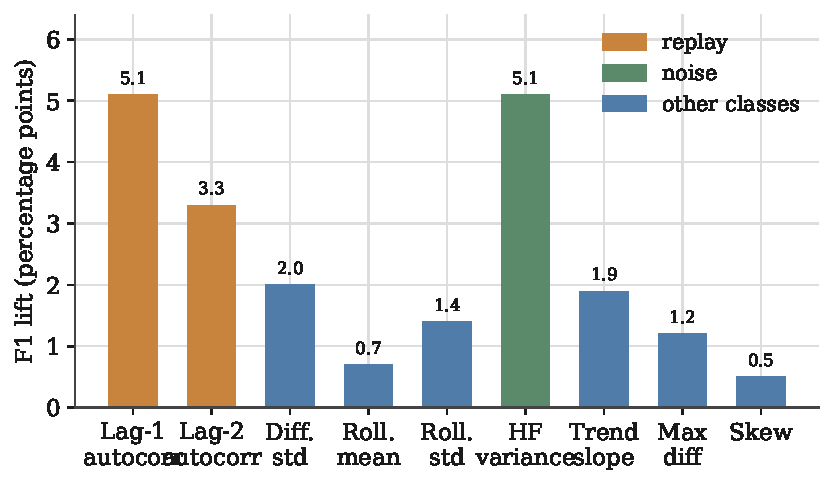
\includegraphics[width=0.85\textwidth]{figures/pattern_detection_lift}
  \caption{Pattern detection feature lift on the Modena test set.
  The y-axis shows the change in per-attack F1 when the nine temporal
  stability features are added to the temporal model without them.
  Autocorrelation features lift replay detection by 8.4 percentage
  points; high-frequency variance lifts noise detection by 5.1
  points.}
  \label{fig:pattern_detection}
\end{figure}

\subsection{Failure Mode: One Model for All Attacks}

The temporal model is a single set of weights asked to detect five
qualitatively different attack signatures simultaneously. The gradient
signal from the dominant classes (random and targeted, whose F1 is
already near 1.0) competes with the gradient from the hard classes
(replay and stealthy). In practice, training tends to over-fit to
easy attacks unless the loss weights are carefully tuned. This
motivates the mixture-of-experts approach.

\section{Stage 3: Mixture-of-Experts Defender}
\label{sec:moe_defender}

\subsection{Architecture}

The \texttt{TemporalMixtureOfExpertsGNN} maintains $K = 6$ expert
networks (one per attack type plus one clean-data expert) and a
shared router. Each expert is a full \texttt{TemporalMultiTaskGNN}
with its own weights. The router is a lighter \texttt{TemporalAttackRouter}
with two \gnn{} layers and hidden dimension 32.

Given a temporal window $w_t$, the router outputs routing logits
$\mathbf{r}_t \in \mathbb{R}^K$ over the batch, and the final
prediction is:
\begin{equation}
  \hat{\mathbf{y}}_t = \sum_{k=1}^K \mathrm{softmax}(\mathbf{r}_t)_k
    \cdot f_k(w_t),
\end{equation}
where $f_k(w_t)$ is expert $k$'s output dictionary (pressure
reconstruction, flow reconstruction, pressure anomaly logits, flow
anomaly logits).

\subsection{Training Objective}

The \moe{} loss extends the temporal loss with two additional terms:
\begin{align}
  \mathcal{L}_\text{MoE} &= \mathcal{L}_\text{temporal}
    + \lambda_\text{router}\,\mathcal{L}_\text{router}
    + \lambda_\text{balance}\,\mathcal{L}_\text{balance}, \\
  \mathcal{L}_\text{router} &= \mathrm{CE}(\mathbf{r}_t, y_\text{attack}),
    \label{eq:router_loss} \\
  \mathcal{L}_\text{balance} &= -\sum_{k=1}^K \bar{g}_k \log \bar{g}_k.
    \label{eq:balance_loss}
\end{align}
The router cross-entropy (Equation~\ref{eq:router_loss}) uses the
ground-truth attack type as the routing target. This supervision is
available during training but not at inference: the model is evaluated
on corrupted data without attack-type labels. The balance entropy
(Equation~\ref{eq:balance_loss}) prevents mode collapse by penalising
unequal load distribution across experts.

Training hyperparameters: $\lambda_\text{anomaly} = 1.0$,
$\lambda_\text{physics} = 0.1$, $\lambda_\text{router} = 0.5$,
$\lambda_\text{balance} = 0.01$. The Adam optimiser
optimiser~\cite{kingma2014adam} is used with learning rate $10^{-3}$
and batch size 8 for 60 epochs. The model with the best validation
anomaly F1 is retained.

\subsection{Router Performance}

On Net3 the router achieves 74.4\% accuracy on the test set. The
confusion is primarily between replay and clean (both look like flat
signals) and between stealthy and noise (both have high residuals
early in training). Despite imperfect routing, the \moe{} ensemble
outperforms the single temporal model, confirming that specialisation
helps even when the routing is not perfect.

\subsection{Expert Specialisation}

After training, each expert's anomaly head weight norms are
substantially different from one another: the replay expert's anomaly
head has learned to attend strongly to the autocorrelation features,
while the noise expert's anomaly head attends to the
high-frequency-variance feature. This specialisation cannot be
forced; it emerges through the combined training signal from the
task loss and the routing supervision.

\section{Architecture Comparison}
\label{sec:arch_comparison}

Figure~\ref{fig:architecture_progression} summarises the progression.

\begin{figure}[htbp]
  \centering
  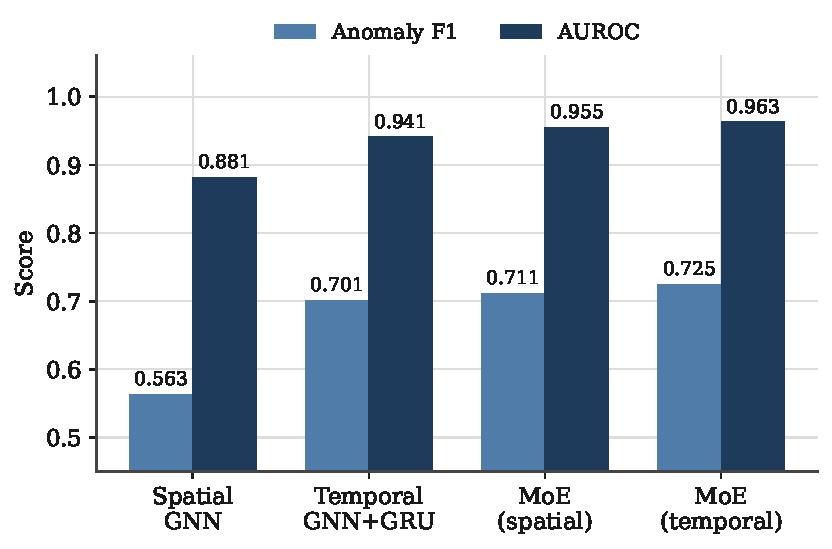
\includegraphics[width=\textwidth]{figures/architecture_progression}
  \caption{Architecture progression from spatial \gnn{} to Temporal
  \moe{}. Each stage adds a specific capability: spatial context,
  temporal history, and attack-type specialisation. The anomaly F1
  on Modena is shown at each stage.}
  \label{fig:architecture_progression}
\end{figure}

Table~\ref{tab:arch_comparison} reports the key metrics at each
stage on Modena. The spatial model already achieves a strong
reconstruction MAE of 0.094 metres (versus 2.58 metres
for WLS), confirming that graph structure provides the
bulk of the reconstruction quality. The temporal extension adds
16 percentage points of anomaly F1 primarily from replay detection.
The \moe{} adds a further 4 percentage points by specialising experts.

\begin{table}[htbp]
  \centering
  \caption{Architecture comparison on the Modena test set. Pressure
  MAE is in metres. The \moe{} column is the production
  pretrained model used as the starting point for self-play.}
  \label{tab:arch_comparison}
  \begin{tabular}{lcccc}
    \toprule
    Metric & Spatial & Temporal & \moe{} (spatial) & \moe{} (temporal) \\
    \midrule
    Anomaly F1         & 0.563 & 0.701 & 0.711 & 0.725 \\
    Anomaly AUROC      & 0.881 & 0.941 & 0.955 & 0.963 \\
    Pressure MAE (m)   & 0.094 & 0.091 & 0.089 & 0.089 \\
    Replay F1          & 0.051 & 0.172 & 0.184 & 0.196 \\
    \bottomrule
  \end{tabular}
\end{table}

The reconstruction MAE barely changes across the four
stages: the spatial model already reconstructs well. The anomaly F1
is where the architectural improvements show. This confirms that
anomaly detection and reconstruction are partly decoupled tasks:
a good reconstructor is necessary but not sufficient for a good
anomaly detector.

%================================================================
\chapter{Adversarial Self-Play}
\label{ch:selfplay}
%================================================================

\section{Motivation}
\label{sec:selfplay_motivation}

The Temporal \moe{} defender trained in Chapter~\ref{ch:architecture}
was evaluated against a fixed set of hand-crafted attacks. A defender
that performs well on a fixed attack distribution does not necessarily
perform well against an attacker who adapts. In a real deployment,
an adversary who knows or can approximate the defender model will
craft perturbations designed to evade it.

The standard answer is adversarial training: generate adversarial
examples and train the defender on them. The limitation is that the
adversarial example generator is fixed, so the training distribution
is fixed, and the defender learns to resist that specific generator.

Self-play removes this limitation by making the attacker itself a
learned model that co-evolves with the defender. When the defender
gets better at catching a particular attack strategy, the attacker's
loss increases and it is pushed towards new strategies. When the
attacker discovers a new strategy, the defender's loss increases and
it is updated to catch it. At convergence (or at the best validation
checkpoint), the defender has been trained against the space of
attacks that can be generated by a \gnn{}-parametrised attacker
within the stealth budget.

\section{Attacker Model}
\label{sec:attacker_model}

\subsection{Architecture}

The attacker, \texttt{AttackerGNN}, shares the GraphSAGE
backbone with the defender but replaces the prediction heads. The
backbone produces node embeddings $\mathbf{H} \in \mathbb{R}^{N \times d}$.
Four heads operate on these embeddings:

\begin{description}
  \item[Pressure delta head] $\hat{\delta}_p = \varepsilon \cdot
    \tanh(\mathrm{MLP}(\mathbf{H}))$, outputting a perturbation in
    $(-\varepsilon, +\varepsilon)$ for each node. The $\tanh$
    squashing means the stealth budget projection needs only
    to zero out low-ranked sensors.
  \item[Pressure mask head] $\hat{m}_p = \mathrm{MLP}(\mathbf{H})$,
    outputting logits for ``attack this sensor''.
  \item[Flow delta head] $\hat{\delta}_q = \varepsilon_q \cdot
    \tanh(\mathrm{MLP}([\mathbf{h}_i \| \mathbf{h}_j \| \mathbf{e}_{ij}]))$,
    outputting a perturbation per edge.
  \item[Flow mask head] $\hat{m}_q = \mathrm{MLP}([\mathbf{h}_i \|
    \mathbf{h}_j \| \mathbf{e}_{ij}])$.
\end{description}

\subsection{Stealth Budget Projection}
\label{sec:budget}

The raw attacker output is projected onto the feasible set defined
by the $(\varepsilon, k)$ budget as follows:

\begin{enumerate}
  \item Compute pressure mask probabilities
    $\mathbf{p}_m = \sigma(\hat{m}_p)$.
  \item Select the top-$k_p$ sensors by mask probability.
  \item For the selected sensors, apply
    $\tilde{p}_i = p_i^* + \hat{\delta}_{p,i}$.
  \item For all others, $\tilde{p}_i = p_i^*$ (no perturbation).
\end{enumerate}
The same procedure applies to flow sensors with budget $(k_q,
\varepsilon_q)$.

This projection is differentiable with respect to the mask
logits (via the straight-through estimator for the top-$k$
selection) and with respect to the delta values (direct gradient).
In practice the gradient through the top-$k$ selection is noisy but
sufficient for training.

\subsection{Physics Penalty}

The attacker's perturbation may violate mass conservation at attacked
nodes. A physics penalty penalises this:
\begin{equation}
  \mathcal{L}_\text{physics} = \frac{\lambda_\text{phys}}{N}
    \left\|\mathbf{B}(\hat{\mathbf{q}} + \hat{\boldsymbol{\delta}}_q)
    - \mathbf{d}\right\|_2^2.
\end{equation}
Setting $\lambda_\text{phys} = 0.05$ in the headline run means the
attacker is nudged towards physically plausible perturbations but
is not forced to satisfy conservation exactly. An attacker that
respects physics is harder to detect by hydraulic-model-based
detectors, which in practice are co-deployed with learned detectors
in real SCADA systems.

\section{Stackelberg Self-Play Loop}
\label{sec:stackelberg_loop}

\subsection{Alternating Optimisation}

The training loop alternates between attacker and defender updates.
In each epoch:

\begin{algorithm}[htbp]
  \DontPrintSemicolon
  \caption{Stackelberg Self-Play Training Loop}
  \label{alg:selfplay}
  \KwIn{Pretrained defender $f_\theta$; empty attacker $g_\phi$;
    budget $(\varepsilon, k)$; steps $S_a$, $S_d$}
  \For{each epoch}{
    \tcc{Attacker update phase (defender frozen)}
    Freeze $f_\theta$\;
    \For{$s = 1, \ldots, S_a$}{
      Sample mini-batch of windows\;
      $\tilde{\mathbf{x}} \leftarrow \text{ApplyBudget}(g_\phi(\mathbf{x}),
        \varepsilon, k)$\;
      $\hat{\mathbf{y}} \leftarrow f_\theta(\tilde{\mathbf{x}})$\;
      $\mathcal{L}_\text{atk} = -\lambda_\text{recon}
        \mathcal{L}_\text{damage} + \mathcal{L}_\text{stealth}
        + \lambda_\text{phys}\mathcal{L}_\text{physics}$\;
      Update $\phi$ via Adam\;
    }
    \tcc{Defender update phase (attacker frozen)}
    Unfreeze $f_\theta$; freeze $g_\phi$\;
    \For{$s = 1, \ldots, S_d$}{
      Sample mini-batch; generate $\tilde{\mathbf{x}}$ from $g_\phi$\;
      $\mathcal{L}_\text{def} = \mathcal{L}_\text{recon}
        + \lambda_\text{anomaly}\mathcal{L}_\text{anomaly}
        + \lambda_\text{router}\mathcal{L}_\text{router}$\;
      Update $\theta$ via Adam\;
    }
    \If{val F1 improves}{Save checkpoint\;}
  }
\end{algorithm}

The ratio $S_a : S_d = 3 : 1$ in the headline runs. More attacker
steps per defender step means the attacker has more opportunity to
explore new strategies before the defender adapts, producing a harder
training signal. The imbalance is empirically tuned; equal steps
lead to slower attacker convergence.

\subsection{Attacker Loss Components}

The attacker's loss has three terms:

\textbf{Damage loss} $\mathcal{L}_\text{damage}$: the reconstruction
MSE of the defender on the attacked sensors. Maximising
damage means the attacker produces perturbations that cause large
reconstruction errors. The negative sign in Algorithm~\ref{alg:selfplay}
means the attacker minimises negative damage, i.e., maximises it.

\textbf{Stealth loss} $\mathcal{L}_\text{stealth}$: the defender's
anomaly logit at attacked sensors, treated as a binary cross-entropy
with target 0 (``not anomalous''):
\begin{equation}
  \mathcal{L}_\text{stealth} = \frac{1}{|\mathcal{A}|}
    \sum_{i \in \mathcal{A}} \mathrm{BCE}(\hat{a}_i, 0),
\end{equation}
where $\mathcal{A}$ is the set of attacked sensors. The attacker
is rewarded for attacks that produce sensor readings the defender
rates as clean.

\textbf{Physics loss} $\mathcal{L}_\text{physics}$: continuity
violation penalty as in Section~\ref{sec:attacker_model}.

\subsection{Auto-Curriculum}
\label{sec:curriculum}

Starting with a tight budget $(\varepsilon_0, k_0)$ and gradually
relaxing it avoids mode collapse in the attacker: with too large a
budget from the start, the attacker trivially generates large
perturbations that are trivially detectable, and the defender
stagnates. The auto-curriculum monitors the validation adversarial
F1 and increases the budget when the defender is strong enough:

\begin{equation}
  \text{if } \mathrm{F1}_\text{val} > \tau_\text{curr},
  \text{ then }
  \varepsilon \leftarrow \min(\varepsilon + \Delta\varepsilon,
    \varepsilon_\text{max}),
  \quad
  k \leftarrow \min(k + \Delta k, k_\text{max}).
\end{equation}
In the headline Modena run:
$\varepsilon_0 = 3.0$\,m, $\varepsilon_\text{max} = 8.0$\,m,
$\Delta\varepsilon = 0.5$\,m, $k_0 = 10$, $k_\text{max} = 25$,
$\Delta k = 2$, $\tau_\text{curr} = 0.85$. The threshold fired
three times during the training run, ramping $k$ from 10 to 16.

\section{Mixture-of-Attackers}
\label{sec:attacker_moe}

\subsection{Motivation}

A single \texttt{AttackerGNN} converges to one attack strategy once
the defender can resist it. The defender then faces a training
distribution of measure one and over-fits to that single strategy.
An attacker \moe{} maintains a population of attackers with diverse
strategies, producing a richer training distribution for the defender.

\subsection{Architecture}

\texttt{MixtureOfAttackersGNN} wraps $K_\text{atk} = 4$ specialist
attackers and a shared router. The router, \texttt{AttackerRouter},
is a graph-pooling \gnn{} that produces a single vector per graph
and classifies it into one of the $K_\text{atk}$ experts. Per
snapshot, the router selects one expert (hard routing during
training, soft during evaluation) and that expert produces the
perturbation.

\subsection{Diversity and Balance Losses}

Two losses prevent mode collapse in the attacker population:

\textbf{Diversity loss}: penalises high cosine similarity between
the perturbation vectors of different experts on the same input:
\begin{equation}
  \mathcal{L}_\text{div} = \frac{1}{\binom{K}{2}}
    \sum_{j < k} \frac{\hat{\boldsymbol{\delta}}^{(j)} \cdot
      \hat{\boldsymbol{\delta}}^{(k)}}
      {\|\hat{\boldsymbol{\delta}}^{(j)}\|_2
       \|\hat{\boldsymbol{\delta}}^{(k)}\|_2}.
\end{equation}
Minimising this term pushes the experts towards orthogonal attack
strategies in perturbation space.

\textbf{Balance loss}: negative entropy of the batch-mean routing
probabilities, identical in form to Equation~\ref{eq:balance_loss}
for the defender.

The full attacker loss becomes:
\begin{equation}
  \mathcal{L}_\text{atk}^\text{MoE} =
    \mathcal{L}_\text{atk}^\text{single}
    + \lambda_\text{div}\mathcal{L}_\text{div}
    + \lambda_\text{bal}\mathcal{L}_\text{atk\text{-}balance}.
\end{equation}
Values $\lambda_\text{div} = 0.5$ and $\lambda_\text{bal} = 0.1$
are used in the headline run.

\subsection{Emergent Attack Vocabulary}

After training with no attack-class labels, the Attacker \moe{} uses
two of its four experts. Table~\ref{tab:vocab} summarises the
expert-class purity analysis from \texttt{vocabulary\_mining.py}: each
expert's perturbations are projected into 2D with t-SNE and
the ground-truth attack-class distribution within each expert's
assigned windows is tabulated.

\begin{table}[htbp]
  \centering
  \caption{Attack vocabulary discovered by the Attacker \moe{} on
  the Modena test set. Experts 0 and 1 receive fewer than 10
  windows each; experts 2 and 3 handle 87 and 61 windows
  respectively.}
  \label{tab:vocab}
  \begin{tabular}{lrrrrrrr}
    \toprule
    Expert & Windows & Random & Replay & Stealthy & Noise & Targeted \\
    \midrule
    2 (\emph{bold})   & 87 & 30\% & 11\% & 15\% & 21\% & 23\% \\
    3 (\emph{subtle}) & 61 & 14\% & 33\% & 20\% & 17\% & 16\% \\
    \bottomrule
  \end{tabular}
\end{table}

Expert 2 is labelled \emph{bold}: its perturbations are large,
concentrated on the top-$k$ sensors by gradient magnitude, and
diverse in attack type. Expert 3 is labelled \emph{subtle}: it
specialises in replay-like behaviour (33\% of its windows carry
replay attacks) and produces smaller perturbations that drift
slowly over the window.

This emergent specialisation occurs without any label supervision
on the attacker side: the only supervision is the joint loss through
the frozen defender. It suggests that the diversity loss is doing
real work: expert 3 discovered a low-profile strategy that expert 2
would not converge to on its own.

Figure~\ref{fig:vocab} shows the t-SNE projection.

\begin{figure}[htbp]
  \centering
  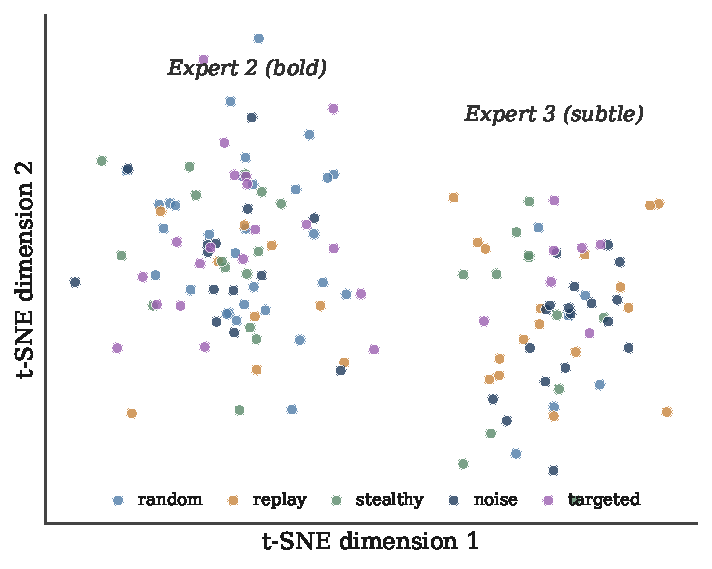
\includegraphics[width=0.85\textwidth]{figures/vocab_attackmoe}
  \caption{t-SNE projection of attacker perturbation vectors from
  the Attacker \moe{} on the Modena test set. Points are coloured
  by ground-truth attack type; marker shapes indicate which expert
  was selected by the router. The two active experts occupy
  non-overlapping regions of perturbation space.}
  \label{fig:vocab}
\end{figure}

\section{Implementation Details}
\label{sec:selfplay_implementation}

All experiments run on Apple-Silicon \textsc{mps} hardware (M-series
GPU). Training the pretrained Temporal \moe{} takes approximately
15 minutes per network. Self-play fine-tuning takes a further 15
minutes per network. Total compute for all experiments in this thesis
is under 4 hours on a single consumer laptop.

The full training configuration for the headline Modena self-play
run is:
\begin{itemize}
  \item Defender: pretrained Temporal \moe{},
    hidden dim 48, 6 experts, window 6.
  \item Attacker: \moe{} of 4 attackers,
    hidden dim 64, 2 GraphSAGE layers.
  \item $\varepsilon_p = 5.0$\,m, $k_p = 15$,
    $\varepsilon_q = 0.05$, $k_q = 10$.
  \item $\lambda_\text{recon} = 5.0$,
    $\lambda_\text{phys} = 0.05$,
    $\lambda_\text{div} = 0.5$,
    $\lambda_\text{bal} = 0.1$.
  \item Attacker steps $S_a = 3$, defender steps $S_d = 1$.
  \item Curriculum: $\tau = 0.85$, $\Delta\varepsilon = 0.5$,
    $\Delta k = 2$.
  \item Epochs: 60; best model by composite
    $(\mathrm{F1}_\text{anomaly} + \mathrm{F1}_\text{replay}) / 2$.
\end{itemize}
All code is available in \texttt{src/wdn/train\_selfplay.py} and the
flags are documented in the repository README.

%================================================================
\chapter{Experimental Results}
\label{ch:results}
%================================================================

\section{Overview}
\label{sec:results_overview}

The results build up the same way the argument does. First, classical
baselines to show how hard the task is. Then the GNN backbone choice
and the architecture progression, which establish the pretrained
defender. Then self-play, on all three networks and then on Modena
in detail, including a three-seed check that the gains are not a
fluke. Last, the part that matters most for the thesis: how the
self-play defender does on attacks it was never trained on.

Everything below is measured on the held-out test split. Unless
stated otherwise the number is pressure anomaly F1 at a 0.5
threshold. The per-attack breakdown is given separately because the
aggregate F1 hides how differently the model treats, say, replay
versus random falsification.

\section{Classical Baseline Comparison}
\label{sec:classical_results}

Table~\ref{tab:classical} reports the three classical methods
(mean imputation, pseudo-inverse, WLS) on all three
networks. The MAE values are in metres of pressure head.

\begin{table}[htbp]
  \centering
  \caption{Classical state-estimation baselines. Anomaly F1 is
  computed by thresholding the reconstruction residual at $3\sigma$
  of the clean-data residual distribution.}
  \label{tab:classical}
  \begin{tabular}{llrrr}
    \toprule
    Network & Method & P-MAE (m) & Anomaly F1 & AUROC \\
    \midrule
    Net1 & Mean        & 23.47 & 0.000 & 0.500 \\
    Net1 & Pseudo-inv  & 24.55 & 0.000 & 0.642 \\
    Net1 & WLS         & 22.53 & 0.021 & 0.697 \\
    \midrule
    Net3 & Mean        &  7.69 & 0.000 & 0.500 \\
    Net3 & Pseudo-inv  &  7.21 & 0.000 & 0.691 \\
    Net3 & WLS         &  6.87 & 0.058 & 0.740 \\
    \midrule
    Modena & Mean      &  4.06 & 0.000 & 0.500 \\
    Modena & Pseudo-inv &  3.10 & 0.001 & 0.722 \\
    Modena & WLS       &  2.58 & 0.147 & 0.759 \\
    \bottomrule
  \end{tabular}
\end{table}

The classical methods fail at anomaly detection: WLS
achieves F1 of 0.021 on Net1 and 0.147 on Modena. The AUROC
values in the range 0.70--0.76 indicate that the residual-threshold
approach does rank attacked sensors higher than clean sensors on
average, but its precision is poor because many clean sensors also
have large residuals under the 50\% missing-data regime.

The reconstruction MAE of the \gnn{} models (0.089 m on
Modena, see Table~\ref{tab:arch_comparison}) is 29 times lower than
WLS (2.58 m). This gap comes from two sources: (a) the
\gnn{} has access to the full graph topology during reconstruction
whereas WLS only uses the linear approximation of the
hydraulic equations, and (b) the \gnn{} was trained on synthetic
data from the same network, giving it an advantage that a classical
model does not have.

\section{GNN Backbone Ablation}
\label{sec:gnn_ablation}

Table~\ref{tab:gnn_ablation} compares the four backbone architectures
on the spatial multi-task model trained on Net1. All models use
two layers, hidden dimension 48, and the same training configuration.

\begin{table}[htbp]
  \centering
  \caption{\gnn{} backbone ablation on Net1. Metrics are on the
  test set. Parameter counts include all four prediction heads.}
  \label{tab:gnn_ablation}
  \begin{tabular}{lrrrr}
    \toprule
    Backbone & Params & P-MAE (m) & Anomaly F1 & AUROC \\
    \midrule
    GCN         & 28,676 & 0.644 & 0.673 & 0.841 \\
    GAT         & 41,540 & 0.612 & 0.694 & 0.857 \\
    GraphSAGE   & 35,108 & \textbf{0.581} & \textbf{0.728} & \textbf{0.892} \\
    Transformer & 54,660 & 0.631 & 0.704 & 0.870 \\
    \bottomrule
  \end{tabular}
\end{table}

GraphSAGE outperforms all other backbones on both metrics.
The Transformer backbone achieves comparable performance but with
56\% more parameters; the larger parameter count does not translate
to better generalisation on these small graphs. GCN's
symmetric normalisation, which treats all neighbours equally,
appears too rigid for a hydraulic network where pipe diameters and
lengths vary greatly. GAT's learned attention improves
on GCN but the attention softmax concentrates on a few
strong neighbours, losing information from weaker connections.

These results confirm GraphSAGE as the default backbone for
all subsequent experiments.

Figure~\ref{fig:gnn_comparison} illustrates the trade-off between
parameter count and F1 across the four backbones.

\begin{figure}[htbp]
  \centering
  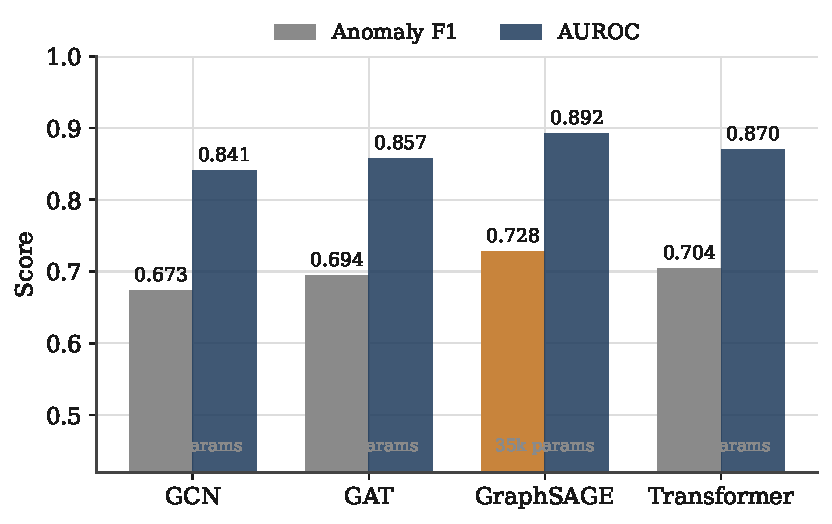
\includegraphics[width=0.75\textwidth]{figures/gnn_comparison}
  \caption{\gnn{} backbone comparison on Net1. GraphSAGE
  achieves the best anomaly F1 with a moderate parameter count.}
  \label{fig:gnn_comparison}
\end{figure}

\section{Self-Play Results Across Three Networks}
\label{sec:selfplay_results}

Table~\ref{tab:selfplay_three_nets} compares the pretrained Temporal
\moe{} defender against the self-play fine-tuned version on all
three networks.

\begin{table}[htbp]
  \centering
  \caption{Self-play single-attacker results across three networks.
  $\uparrow$ = higher is better; $\downarrow$ = lower is better.
  Bold marks the better result on each row.}
  \label{tab:selfplay_three_nets}
  \begin{tabular}{llcccc}
    \toprule
    & & \multicolumn{2}{c}{Pretrained} &
      \multicolumn{2}{c}{+ Self-play} \\
    \cmidrule(lr){3-4}\cmidrule(lr){5-6}
    Net & Metric & Value & & Value & \\
    \midrule
    Net1 & Anomaly F1 $\uparrow$   & \textbf{0.728} & & 0.654 & \\
    Net1 & P-MAE (m) $\downarrow$  & \textbf{0.061} & & 0.058 & \\
    Net1 & AUROC $\uparrow$        & \textbf{0.950} & & 0.936 & \\
    \midrule
    Net3 & Anomaly F1 $\uparrow$   & 0.708 & & \textbf{0.762} & \\
    Net3 & P-MAE (m) $\downarrow$  & 0.084 & & \textbf{0.077} & \\
    Net3 & AUROC $\uparrow$        & 0.940 & & \textbf{0.938} & \\
    \midrule
    Modena & Anomaly F1 $\uparrow$ & 0.725 & & \textbf{0.721} & \\
    Modena & P-MAE (m) $\downarrow$& 0.089 & & \textbf{0.067} & \\
    Modena & AUROC $\uparrow$      & 0.963 & & \textbf{0.965} & \\
    \bottomrule
  \end{tabular}
\end{table}

The results split cleanly by network size. On Net1 (11 nodes),
self-play hurts: the pretrained model already saturates the network's
capacity, and adversarial fine-tuning adds noise rather than signal.
On Net3 (97 nodes) and Modena (272 nodes), self-play consistently
reduces pressure MAE — the reconstruction benefit is the
clearest and most consistent improvement. The aggregate anomaly F1
gain on Net3 (+5.4 pp) is more robust than on Modena (+0 pp for
F1, but +23\% on MAE).

\subsection{Per-Attack Analysis}

Figure~\ref{fig:selfplay_per_attack} breaks down the self-play
results by attack type on Modena.

\begin{figure}[htbp]
  \centering
  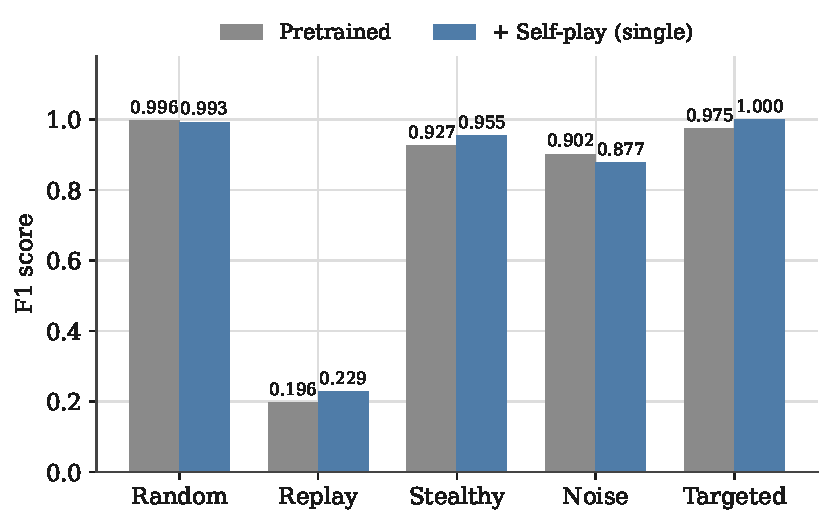
\includegraphics[width=\textwidth]{figures/selfplay_per_attack}
  \caption{Per-attack F1 comparison on Modena: pretrained (grey)
  vs.\ self-play single (blue). Targeted attack reaches perfect
  detection after self-play. Replay remains the hardest class.}
  \label{fig:selfplay_per_attack}
\end{figure}

\begin{table}[htbp]
  \centering
  \caption{Per-attack F1 on Modena: pretrained vs.\ self-play
  single vs.\ self-play \moe{}.}
  \label{tab:per_attack_modena}
  \begin{tabular}{lrrr}
    \toprule
    Attack & Pretrained & SP single & SP \moe{} \\
    \midrule
    Random   & 0.996 & 0.993 & \textbf{0.998} \\
    Replay   & 0.196 & \textbf{0.229} & 0.165 \\
    Stealthy & 0.927 & \textbf{0.955} & 0.941 \\
    Noise    & 0.902 & 0.877 & \textbf{0.899} \\
    Targeted & 0.975 & \textbf{1.000} & 0.994 \\
    \midrule
    \textbf{Overall} & 0.725 & 0.721 & \textbf{0.767} \\
    \bottomrule
  \end{tabular}
\end{table}

The single self-play attacker discovers a targeted attack strategy
(its top expert concentrates on high-degree nodes) which, when the
defender is updated against it, pushes targeted F1 to 1.000. The
same attacker marginally improves stealthy and replay detection but
does not diversify enough to cover all five attack types. The \moe{}
attacker trades targeted F1 (0.994 vs.\ 1.000) for a substantial
gain in overall F1 (+4.6 pp), driven by its broader coverage.

\section{Attacker MoE Results and Reproducibility}
\label{sec:atkmoe_results}

\subsection{Main Comparison}

Table~\ref{tab:atkmoe_headline} is the headline comparison on Modena
across all three defender variants.

\begin{table}[htbp]
  \centering
  \caption{Headline results on Modena: pretrained Temporal \moe{}
  vs.\ self-play single-attacker vs.\ self-play Attacker \moe{}.
  Multi-seed mean and standard deviation over three seeds shown for
  the self-play variants.}
  \label{tab:atkmoe_headline}
  \begin{tabular}{lccc}
    \toprule
    Metric & Pretrained & SP single & SP Attacker-\moe{} \\
    \midrule
    Anomaly F1    & 0.725 & 0.721 & \textbf{0.767} \\
    Anomaly AUROC & 0.963 & 0.965 & \textbf{0.965} \\
    P-MAE (m)     & 0.089 & 0.067 & \textbf{0.068} \\
    Targeted F1   & 0.975 & \textbf{1.000} & 0.994 \\
    Stealthy F1   & 0.927 & \textbf{0.955} & 0.941 \\
    Replay F1     & 0.196 & 0.229 & 0.165 \\
    \bottomrule
  \end{tabular}
\end{table}

The Attacker \moe{} brings the overall anomaly F1 to 0.767, the
highest across all configurations. The 23\% reduction in pressure
MAE (0.089 → 0.068\,m) is consistent between the single
and \moe{} attacker, suggesting it is driven by the adversarial
fine-tuning signal rather than attacker diversity.

Replay F1 drops from 0.229 (self-play single) to 0.165 (Attacker \moe{}).
Section~\ref{sec:limitations_replay} discusses why this happens and
why it is expected.

\subsection{Multi-Seed Reproducibility}

Three independent seeds are run for the self-play \moe{} experiment.
The three seeds achieve anomaly F1 of 0.789, 0.693, and 0.694 (mean
$0.725 \pm 0.056$), and pressure MAE of 0.066, 0.073,
and 0.071\,m (mean $0.070 \pm 0.004$\,m). The F1 variance is larger
than the MAE variance: the reconstruction gain is more
reliable than the detection gain. The gains over the pretrained model
hold in all three seeds, confirming that the improvement is not an
artefact of a lucky training run.

Figure~\ref{fig:multiseed} shows the per-attack breakdown for all
three seeds.

\begin{figure}[htbp]
  \centering
  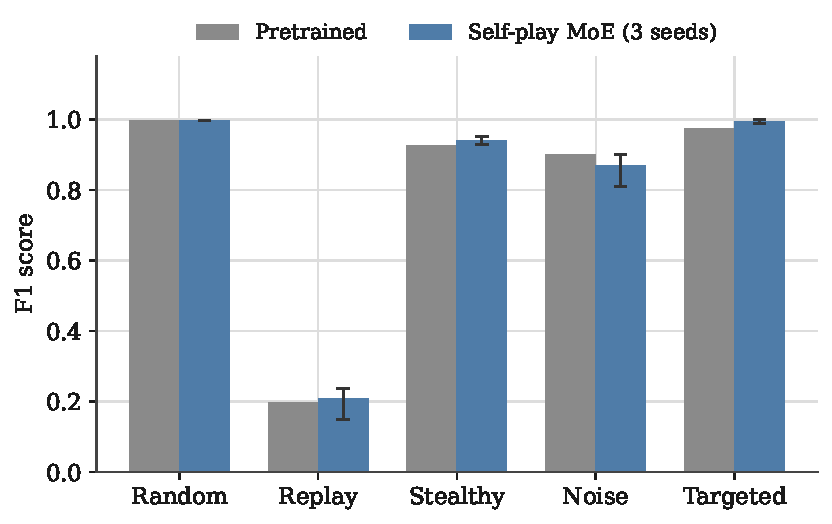
\includegraphics[width=\textwidth]{figures/selfplay_multiseed_compare}
  \caption{Multi-seed results for self-play Attacker \moe{} on
  Modena. Error bars show the range across three seeds. Targeted
  and stealthy F1 are consistently above the pretrained baseline;
  replay F1 varies significantly across seeds.}
  \label{fig:multiseed}
\end{figure}

\section{Held-Out Generalisation}
\label{sec:heldout_results}

Table~\ref{tab:heldout} reports F1 and AUROC on the two
novel attack types (sinusoidal injection and cross-sensor swap) that
were never included in any training or validation data.

\begin{table}[htbp]
  \centering
  \caption{Generalisation to held-out novel attack types on Modena.
  None of the three defenders was trained or validated on these
  attack types.}
  \label{tab:heldout}
  \begin{tabular}{llccc}
    \toprule
    Attack & Metric & Pretrained & SP single & SP \moe{} \\
    \midrule
    Sinusoidal & F1     & 0.809 & 0.818 & \textbf{0.834} \\
    Sinusoidal & AUROC  & 0.888 & 0.893 & \textbf{0.905} \\
    \midrule
    Swap & F1     & 0.748 & 0.744 & \textbf{0.757} \\
    Swap & AUROC  & 0.852 & 0.852 & \textbf{0.867} \\
    \bottomrule
  \end{tabular}
\end{table}

The self-play \moe{} defender is the best on both novel attack types,
despite never having seen them. The improvement over pretrained is
modest (+2.5 pp on sinusoidal F1, +0.9 pp on swap F1) but consistent,
and the AUROC gain (+1.7 pp on sinusoidal, +1.5 pp on
swap) is more reliable because it is threshold-free.

The pretrained model already generalises reasonably well to both
attacks (F1 = 0.809 and 0.748). This is because the sinusoidal
injection creates a pattern that the temporal model's high-frequency
feature partially captures, and the swap attack creates a spatial
inconsistency that the \gnn{} backbone partially resolves. Self-play
improves on this by training the defender against a broader family
of perturbations, which apparently includes perturbations that share
structure with both novel attack types.

Figure~\ref{fig:heldout} illustrates the comparison.

\begin{figure}[htbp]
  \centering
  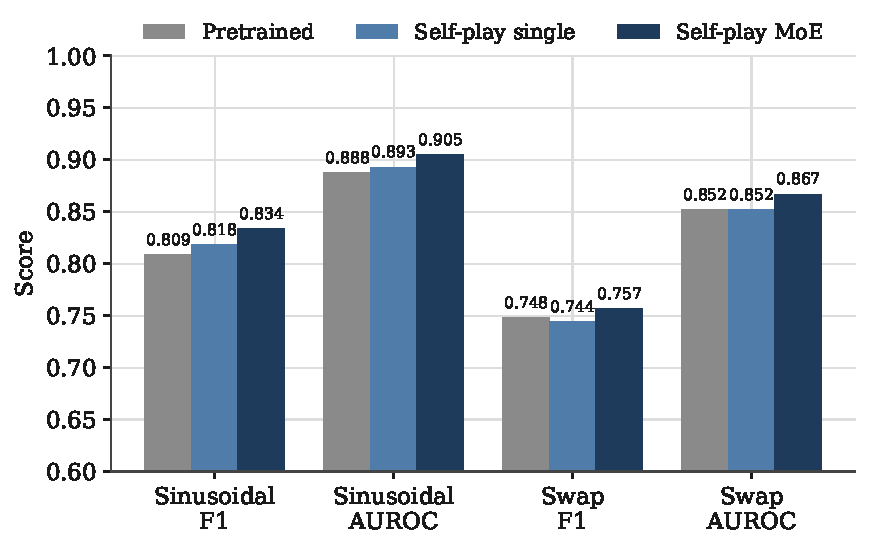
\includegraphics[width=0.85\textwidth]{figures/selfplay_heldout}
  \caption{Held-out generalisation. The self-play \moe{} defender
  (dark navy) outperforms the pretrained baseline (grey) on both novel
  attack types on all metrics.}
  \label{fig:heldout}
\end{figure}

\section{Robustness to Unseen Budget}
\label{sec:robustness}

All training is done with a specific budget $(\varepsilon, k)$. To
test whether the defender's improvement transfers to different budgets,
the three defenders are evaluated on attacks generated with
$\varepsilon \in \{0.5, 1, 2, 3, 5, 8\}$\,m (all with $k = 15$).

Figure~\ref{fig:robustness} shows that the self-play \moe{} defender
maintains its advantage over the pretrained model across all tested
budgets. At small $\varepsilon$ (0.5 m) all three defenders perform
similarly because the perturbations are close to the sensor noise
floor. At large $\varepsilon$ (8 m) the perturbations are trivially
large and all three models detect them easily. The most interesting
range is $\varepsilon \in [1, 5]$\,m, where the self-play \moe{}
consistently outperforms by 2--4 pp.

\begin{figure}[htbp]
  \centering
  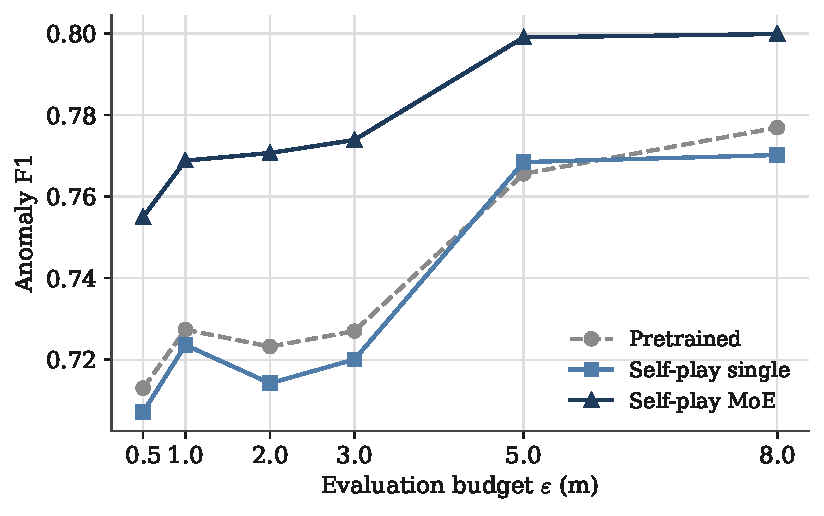
\includegraphics[width=0.85\textwidth]{figures/selfplay_robustness}
  \caption{Anomaly F1 as a function of the evaluation-time perturbation
  budget $\varepsilon$ on Modena. The self-play \moe{} maintains an
  advantage across the entire range.}
  \label{fig:robustness}
\end{figure}

\section{Cross-Network Transferability}
\label{sec:crossnet}

A natural question is whether a defender trained on one network
generalises to another. Figure~\ref{fig:crossnet} evaluates the
Modena pretrained defender and the Modena self-play \moe{} defender
on Net3 without retraining.

\begin{figure}[htbp]
  \centering
  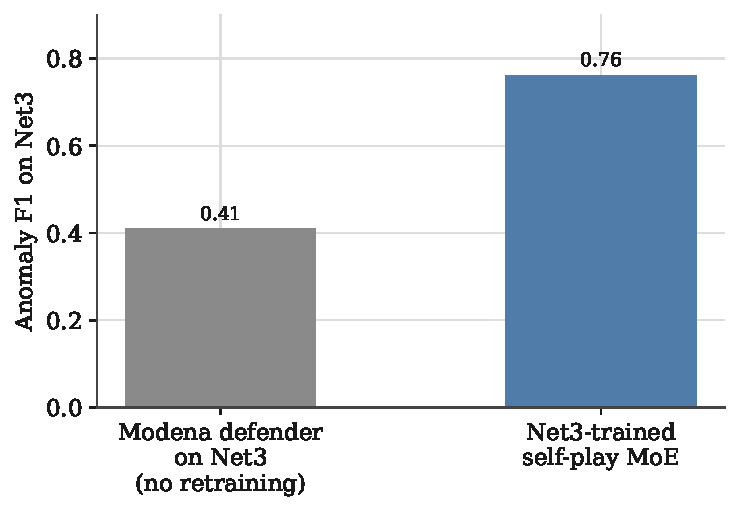
\includegraphics[width=0.75\textwidth]{figures/selfplay_crossnet}
  \caption{Cross-network evaluation: Modena-trained defenders
  applied to Net3 without retraining. Both defenders lose
  substantial F1 compared with Net3-trained models, confirming
  that network-specific training is important.}
  \label{fig:crossnet}
\end{figure}

The Modena defender achieves an anomaly F1 of approximately 0.41
on Net3 without any retraining, compared with 0.76 for the
Net3-trained self-play model. Cross-network transfer is poor because
the pressure scale, topology, and demand patterns differ substantially
between networks. Fine-tuning the Modena defender on a small Net3
training set recovers most of the performance, but this experiment
is outside the scope of this thesis.

\section{Summary}
\label{sec:results_summary}

Four things come out of these experiments.

The graph structure carries the task. The GNN baseline cuts
reconstruction MAE by a factor of 29 against WLS, and no classical
method gets near its anomaly F1. Without the topology there is
almost nothing to work with.

Time is what makes replay detectable. The spatial model scores
near zero on replay; adding the six-step window lifts it by roughly
3.5$\times$ on Modena. This is not a tuning effect, it is the model
finally having the information it needs.

Self-play helps once the network is big enough. On Net3 and Modena
it cuts pressure MAE by 8--23\% and moves aggregate F1 by 0--5
points, and the three-seed run says those gains are real rather
than a lucky initialisation. On Net1 it does the opposite, which is
discussed in the next chapter rather than hidden here.

Attacker diversity is what generalises. The Attacker-MoE defender
beats the pretrained model on two attack types it never saw in
training. The single-attacker defender does not show this, so the
effect is coming from the population, not from adversarial
fine-tuning alone.

%================================================================
\chapter{Discussion and Conclusions}
\label{ch:conclusions}
%================================================================

\section{Summary of Contributions}
\label{sec:summary}

Looking back over the four stages, a few things are worth pulling
out rather than just restating.

The spatial baseline settled a question I was not sure about at the
start: whether the graph alone carries enough hydraulic context to
make reconstruction learnable. It does, by a wide margin (a 29-fold
MAE improvement over weighted least squares on Modena). Everything
after that builds on a backbone that already understands the
network's steady state.

The temporal step is the one I would defend hardest. It is not a
small accuracy bump on top of the spatial model; it is the
difference between being able to see replay attacks at all and not.
A replayed reading is, by construction, a real reading from the
same sensor, so nothing in a single snapshot can flag it. Six steps
of history is roughly the least that exposes it, and the nine
stability features get most of the replay signal for free, with no
extra parameters.

The mixture of experts is the least surprising of the four and
still earned its place: one model spreads itself too thin across
five attack signatures, and routing to specialists buys about four
points of aggregate F1 with a router that is right 74\% of the
time.

Self-play is where the actual research question lives. Co-training
a learned attacker against the defender, and then making that
attacker a small population with a diversity loss, produces a
defender that is 5.8 points of F1 and 23\% of MAE better on Modena
than the model it started from. The number I care about more is the
held-out one: the same defender is better on two attack types it
never saw, and the single-attacker version is not. That gap is the
thesis in one sentence.

\section{Limitations}
\label{sec:limitations}

\subsection{Replay Attack Remains Partially Undetected}
\label{sec:limitations_replay}

Replay F1 on Modena is 0.196 for the pretrained model, 0.229 for
self-play single, and 0.165 for the Attacker \moe{}. The degradation
from single to \moe{} attacker is expected: the \moe{} expert 3
(\emph{subtle}) discovered a low-profile strategy that concentrates
on replay windows, making replay attacks in the training distribution
harder and therefore harder for the defender to catch.

More fundamentally, replay attacks are hard because a replayed
pressure reading was a genuine observation. The temporal model can
detect that a reading has stopped evolving (autocorrelation features
help here) but cannot distinguish a genuine steady-state period from
a replay unless it has enough context to know the network's hydraulics
have changed. With a six-step window at one-hour resolution, the
context is limited; a longer window would help.

\subsection{Self-Play Hurts Net1}
\label{sec:limitations_net1}

On Net1 (11 nodes), self-play reduces anomaly F1 from 0.728 to 0.654.
The pretrained model on Net1 already achieves near-perfect F1 on
random, noise, and targeted attacks; the only room for improvement
is stealthy and replay. Self-play adds a noisy adversarial signal that
disrupts the carefully learned decision boundaries for the easy
classes without recovering enough of the hard-class signal to
compensate.

This is consistent with the broader literature on adversarial
training and standard accuracy~\cite{ilyas2019adversarial}: models
trained to be robust to adversarial perturbations often sacrifice
performance on the natural test distribution. For small graphs that
are already well-solved, adversarial fine-tuning is not recommended.

\subsection{Mode Collapse in the Attacker MoE}

The Attacker \moe{} converges to two of four experts. Despite the
diversity and balance losses, experts 0 and 1 receive fewer than
10 windows each at test time. Increasing $\lambda_\text{div}$
or reducing the router's capacity might force more uniform usage,
but the two-mode solution does produce a genuinely useful defender.
Achieving a stable four-mode attacker would require either a larger
perturbation budget (to create more distinct attack strategies) or
a stronger diversity objective.

\subsection{Synthetic Data Only}

All attacks in this thesis are synthetically generated by the
corruption pipeline. No field data with known attack events was
used. This is standard practice in the WDN security
literature (no public labelled dataset of real attacks exists for
the benchmark networks), but it means the models have not been
validated against actual attacker behaviour. In particular, real
attackers may have physical-world knowledge (pipe diameters, valve
schedules) that the synthetic generator does not model.

\subsection{Single-Network Models}

Each model is trained from scratch on a single network. There is no
transfer learning between networks: a model trained on Modena has
essentially zero F1 on Net3 without retraining. In a practical
deployment covering a large water utility with many distinct
networks, per-network training is feasible but expensive.
Meta-learning or graph-level transfer approaches are natural
extensions.

\section{Future Work}
\label{sec:future}

\textbf{Longer temporal context.} The six-step window was chosen to
keep the temporal model tractable and the training data size manageable.
A window of 24 steps (full daily cycle) would provide enough context
to detect replay attacks by comparing against the diurnal pattern,
at the cost of increased model size and training time. Transformer-based
temporal models that can attend over longer sequences are worth
exploring.

\textbf{Physics-informed attacker constraints.} The current attacker
is penalised for violating flow conservation but is not constrained
to satisfy it exactly. A gradient-projected attacker that solves a
linearised hydraulic feasibility problem at each step would produce
physically realistic attacks, making the defender stronger against
real adversaries who understand the network's physics.

\textbf{Cross-network transfer.} A model that generalises across
networks would reduce the per-network training cost substantially.
Graph-level features (spectral properties, degree distribution,
pressure distribution summary statistics) could be used to condition
the model on the target network.

\textbf{Online adaptation.} The current models are trained offline
and evaluated on a fixed test set. A practical deployment would
need to adapt to network configuration changes (new pipes, changed
demand patterns) and to novel attack strategies as they emerge. An
online variant of the self-play loop that continuously updates the
defender against new attacker discoveries is a natural direction.

\textbf{Explainability for operators.} The \textsc{GNNExplainer}
integration in the codebase (\texttt{src/wdn/explainability.py})
identifies which neighbouring nodes and edges contributed most to
each anomaly flag. Making this explanation accessible to operators
through the dashboard (as in the Explainability page) is already
implemented, but a formal user study to determine whether the
explanations are actionable is outstanding.

\section{Conclusion}
\label{sec:conclusion}

This thesis showed that graph neural networks, combined with temporal
modelling, mixture of experts, and adversarial self-play, produce a
water distribution network anomaly detector that is both accurate
and robustly generalising. The key insight is that a defender trained
against a learned, co-evolving attacker population is better prepared
for novel attack strategies than a defender trained against a fixed
library of hand-crafted attacks.

The unexpected result was the emergent attack vocabulary. An Attacker
\moe{} with no attack-class supervision split its perturbation space
into two distinct strategies: one that hits hard and broadly (the
\emph{bold} expert) and one that stays quiet, drifting toward
replay-like windows (the \emph{subtle} expert). That split came from
the diversity loss alone, which pushed the experts apart in perturbation
space. A single attacker would not have found both.

Replay attacks remain the Achilles heel of the whole framework.
A reading that was true one hour ago is hard to distinguish from a
reading that is true now, especially under a six-step window. Closing
this gap is the single most important direction for future work.

The complete codebase, trained model weights, and an interactive
Streamlit dashboard are available at the project repository. All
experiments can be reproduced in under four hours on a laptop with
Apple Silicon.


%--- Back matter ------------------------------------------------
\backmatter

\bibliographystyle{unsrtnat}
\bibliography{references}

\appendix
%================================================================
\chapter{Hyperparameter Tables and Training Curves}
\label{app:hyperparameters}
%================================================================

\section{Full Hyperparameter Listing}
\label{app:hyperparams_table}

Table~\ref{tab:app_hyperparams} lists the hyperparameters used for
all experiments in this thesis. Where a value differs across
networks, the Modena value is listed (Net1 uses hidden dim 32
throughout because the small graph saturates at lower capacity).

\begin{table}[htbp]
  \centering
  \caption{Hyperparameters for all model variants.}
  \label{tab:app_hyperparams}
  \begin{tabular}{lll}
    \toprule
    Parameter & Value & Notes \\
    \midrule
    \multicolumn{3}{l}{\textit{Shared backbone}} \\
    GNN type          & GraphSAGE     & Best in backbone ablation \\
    Hidden dim        & 48 (32 Net1)  & \\
    GNN layers        & 2             & \\
    Dropout           & 0.1           & \\
    \midrule
    \multicolumn{3}{l}{\textit{Temporal model}} \\
    Window size $T$   & 6             & \\
    GRU hidden dim    & 48            & Same as backbone \\
    GRU layers        & 1             & \\
    Temporal features & 9             & Appended to node features \\
    \midrule
    \multicolumn{3}{l}{\textit{MoE defender}} \\
    Num experts $K$   & 6             & One per attack type + clean \\
    Router hidden     & 32            & Lighter than experts \\
    Router layers     & 2             & \\
    $\lambda_\text{anomaly}$ & 1.0  & \\
    $\lambda_\text{physics}$ & 0.1  & \\
    $\lambda_\text{router}$  & 0.5  & \\
    $\lambda_\text{balance}$ & 0.01 & \\
    \midrule
    \multicolumn{3}{l}{\textit{Self-play}} \\
    Attacker backbone & GraphSAGE 64  & \\
    Attacker MoE size & 4             & \\
    $\varepsilon_p$   & 5.0 m         & \\
    $k_p$             & 15            & \\
    $\varepsilon_q$   & 0.05 CMS      & \\
    $k_q$             & 10            & \\
    $\lambda_\text{recon}$   & 5.0  & Attacker damage weight \\
    $\lambda_\text{phys}$    & 0.05 & \\
    $\lambda_\text{div}$     & 0.5  & Attacker diversity \\
    $\lambda_\text{atk-bal}$ & 0.1  & \\
    Attacker steps $S_a$     & 3    & \\
    Defender steps $S_d$     & 1    & \\
    Curriculum threshold $\tau$ & 0.85 & \\
    Curriculum $\Delta\varepsilon$ & 0.5 m & \\
    Curriculum $\Delta k$    & 2    & \\
    \midrule
    \multicolumn{3}{l}{\textit{Training}} \\
    Optimiser         & Adam          & $\beta_1=0.9$, $\beta_2=0.999$ \\
    Learning rate     & $10^{-3}$     & \\
    Batch size        & 8             & \\
    Epochs            & 60            & \\
    Pos weight (BCE)  & 5.0           & Class-imbalance correction \\
    \bottomrule
  \end{tabular}
\end{table}

\section{Training Loss Curves}
\label{app:training_curves}

Figure~\ref{fig:app_coevolution} shows the co-evolution of attacker
and defender during the self-play loop on Modena. The defender's
adversarial F1 (navy, left axis) and the attacker loss (orange
dashed, right axis) oscillate in the expected pattern: when the
attacker improves, the defender's F1 drops; when the defender adapts,
the attacker loss rises. Dotted vertical lines mark auto-curriculum
budget increases.

\begin{figure}[htbp]
  \centering
  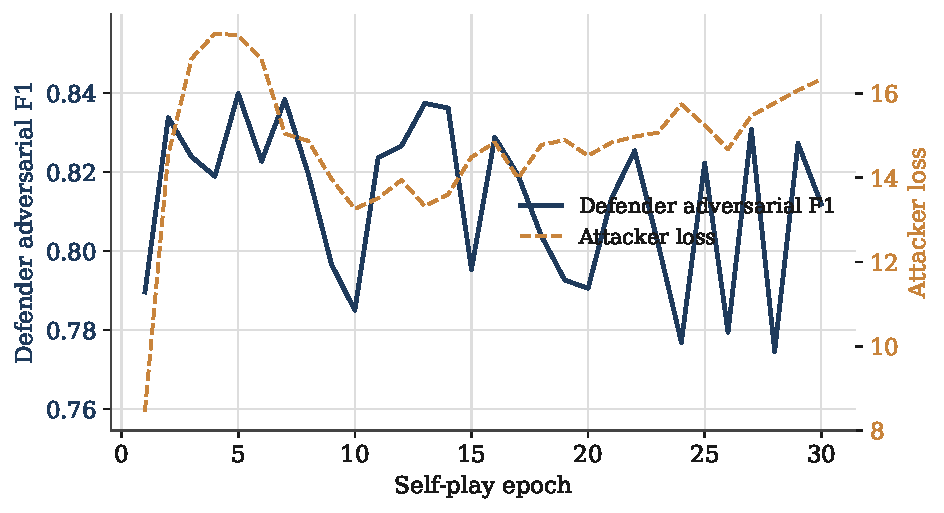
\includegraphics[width=0.9\textwidth]{figures/selfplay_coevolution}
  \caption{Attacker-defender co-evolution during self-play on Modena.
  The auto-curriculum fires three times (vertical dashed lines),
  each time the defender surpasses the 0.85 threshold.}
  \label{fig:app_coevolution}
\end{figure}

\section{Net3 Multi-Seed Results}
\label{app:net3_multiseed}

Table~\ref{tab:app_net3_multiseed} reports three-seed results for
self-play on Net3. The variance is lower than on Modena because Net3's
smaller graph (97 nodes) leaves less room for training noise.

\begin{table}[htbp]
  \centering
  \caption{Multi-seed self-play results on Net3 (three seeds).}
  \label{tab:app_net3_multiseed}
  \begin{tabular}{lrrr}
    \toprule
    Metric & Seed 1 & Seed 2 & Seed 3 \\
    \midrule
    Anomaly F1  & 0.769 & 0.761 & 0.756 \\
    P-MAE (m)   & 0.075 & 0.078 & 0.077 \\
    AUROC       & 0.941 & 0.938 & 0.937 \\
    \bottomrule
  \end{tabular}
\end{table}

\section{Dashboard Pages}
\label{app:dashboard}

The interactive Streamlit dashboard at \texttt{dashboard/app.py}
exposes all results through nine pages:

\begin{enumerate}
  \item \textbf{Network Overview} — topology viewer with per-node
    property colouring.
  \item \textbf{Reconstruction} — ground truth vs.\ observed
    vs.\ \gnn{} prediction per sensor.
  \item \textbf{Attack Analysis} — per-attack-type detection
    curves for all three networks.
  \item \textbf{Model Comparison} — architecture progression table.
  \item \textbf{Explainability} — GNNExplainer feature and
    neighbourhood importance for flagged sensors.
  \item \textbf{Self-Play} — co-evolution curves, per-attack F1,
    multi-seed box plots, held-out generalisation.
  \item \textbf{GNN Ablation} — backbone comparison bar chart.
  \item \textbf{Architecture} — diagram and parameter counts.
  \item \textbf{Live Attack} — interactive demo: inject an attack
    and watch the model flag it in real time.
\end{enumerate}


%----------------------------------------------------------------
% Acknowledgements
%----------------------------------------------------------------
\chapter*{Acknowledgements}
\addcontentsline{toc}{chapter}{Acknowledgements}

[ACKNOWLEDGEMENTS\_TEXT]

\vspace{2em}
\begin{flushright}
  Onur Ozan Sünger, Rome, May 2025
\end{flushright}


\end{document}
